% Style template ines (july 2015)
\documentclass[ngerman]{zhawines}

% Include
\usepackage[ngerman]{babel}
\usepackage{scrpage2}
\usepackage{listings}
\usepackage{amsmath}
\usepackage[squaren]{SIunits}
\usepackage{graphicx}
\usepackage{array}
\usepackage{todonotes}
\usepackage{float}
\usepackage[toc,page]{appendix}
\usepackage[autostyle=true,german=quotes]{csquotes} % quotes
\usepackage{cite}

%\usepackage[latin1]{inputenc}    %Umlaute

%\renewcommand{\contentsname}{Inhaltsverzeichnis}

%---------------------------------------------------------------------
\begin{document}

	\hbadness 10000
	\author{Katrin B�chli }
	\betreuer{Prof. Hans-Joachim Gelke }
	\betreuer{Dr. Matthias Rosenthal }
	\title{PA15\_gelk\_1 Polyphonic DDS Synthesizer mit MIDI Steuerung}
	\subtitle{PA15\_gelk\_1 Polyphonic DDS Synthesizer mit MIDI Steuerung}
	\email{katrin.baechli@zhaw.ch}


%	\maketitle
	
	\headings
	
	
	
	% To Do-Liste 
	\listoftodos     % TO DEL am Ende
	
	%%%%%%%%%%%%%%%%%%%%%%%%%%%%%%%%%%%%%%%%%%%%%%%%%%%%%%%%%%%%%%%%%
%  _____       ______   ____									%
% |_   _|     |  ____|/ ____|  Institute of Embedded Systems	%
%   | |  _ __ | |__  | (___    Wireless Group					%
%   | | | '_ \|  __|  \___ \   Zuercher Hochschule Winterthur	%
%  _| |_| | | | |____ ____) |  (University of Applied Sciences)	%
% |_____|_| |_|______|_____/   8401 Winterthur, Switzerland		%
%																%
%%%%%%%%%%%%%%%%%%%%%%%%%%%%%%%%%%%%%%%%%%%%%%%%%%%%%%%%%%%%%%%%%

\chapter*{Zusammenfassung}


Die hardwarenahe Programmiersprache VHDL ist ein wichtiger Bestandteil der digitalen Signalverarbeitung. Die Projektarbeit setzt zwei unabhängige Aufgaben in VHDL um.

\begin{itemize}
\item Bilden zweier hardwarenahen Fehlerquellen: \textit{Glitches} und \textit{Metastability}
	\item Implementation eines \textit{MIDI Interfaces}, dessen Entwicklung auf einer \textit{textbasierten Test Bench} basiert.
\end{itemize} 

Durch das Verlängern der Pfade einzelner Signale auf einem Cyclon3 II-FPGA werden \textit{Glitches} künstlich herbeigeführt. Da einzelne Werte verzögert eintreffen und verarbeitet der asynchrone \textit{Decoder} falsche Werte. Falsche Signale gelangen auf die Leitung und sogenannte Glitches entstehen. 

Der metastabilen Zustand in einem System entsteht, durch das Verletzen der Setup und Hold Time. Forciert ist dies durch zwei unterschiedliche Takte zweier VHDL-Logik-Blöcke, deren Takt-Phasen nicht übereinstimmen. Das Ausgangssignal des ersten Logik-Blocks ist als asynchroner Impuls auf den zweiten Logik-Block geführt, der eine \textit{Finite State Machine} enthält. Dekodiert die FSM keinen definierten Zustand, befindet sich das System in einen undefinierten Zustand. Metastabilität trifft ein.

Der zweiten Teil der Projektarbeit beinhaltet ein \textit{MIDI Interface}, das Polyphonie detektiert. Die textbasierte \textit{Test Bench} begleitet die Entwicklung des \textit{MIDI Controller}. Das \textit{MIDI Interface} detektiert die \textit{Status Bytes} NOTE ON, NOTE OFF und POLYPHONY und die VHDL-Einheit \textit{Polyphony Out} gibt 10 gedrückte Noten parallel aus.
		
	%%%%%%%%%%%%%%%%%%%%%%%%%%%%%%%%%%%%%%%%%%%%%%%%%%%%%%%%%%%%%%%%%
%  _____       ______   ____									%
% |_   _|     |  ____|/ ____|  Institute of Embedded Systems	%
%   | |  _ __ | |__  | (___    Wireless Group					%
%   | | | '_ \|  __|  \___ \   Zuercher Hochschule Winterthur	%
%  _| |_| | | | |____ ____) |  (University of Applied Sciences)	%
% |_____|_| |_|______|_____/   8401 Winterthur, Switzerland		%
%																%
%%%%%%%%%%%%%%%%%%%%%%%%%%%%%%%%%%%%%%%%%%%%%%%%%%%%%%%%%%%%%%%%%

\chapter*{Abstract}\label{chap.abstract}

???
ou  ou englisch....  mhhhmmmmmmm		
	%%%%%%%%%%%%%%%%%%%%%%%%%%%%%%%%%%%%%%%%%%%%%%%%%%%%%%%%%%%%%%%%%
%  _____       ______   ____									%
% |_   _|     |  ____|/ ____|  Institute of Embedded Systems	%
%   | |  _ __ | |__  | (___    Wireless Group					%
%   | | | '_ \|  __|  \___ \   Zuercher Hochschule Winterthur	%
%  _| |_| | | | |____ ____) |  (University of Applied Sciences)	%
% |_____|_| |_|______|_____/   8401 Winterthur, Switzerland		%
%																%
%%%%%%%%%%%%%%%%%%%%%%%%%%%%%%%%%%%%%%%%%%%%%%%%%%%%%%%%%%%%%%%%%

\chapter*{Vorwort}\label{chap.vorwort}
an Alexey: Bitte hier auf inhaltliche Richtigkeit prüfen. Brauche es erst am Do
korrekt ...

Meine Motivation ist das vertiefte Kennenlernen der Sprache VHDL. Diese hardwarenahe Sprache beinhaltet mit der kombinatorischen Logik und der auch nicht sequentiellen Prozessverarbeitung Eigenheiten, mit denen ich Umgehen lernen wollte.

In der Projektarbeit waren es exakt diese Punkte, mit denen ich viel Zeit durch Debuggen verbrachte. Doch gerade so, ist mir nun diese Art der Programmierung vertrauter geworden und ich freue mich, auf kommende VHDL-Projekte.

Ich möchte Prof. Hans-Joachim Gelke meinen Dank aussprechen. Er legte den Fokus immer wieder auf die kombinatorische Logik und die Konsequenz des Codes, für das Umsetzen in der Hardware. Ebenfalls möchte ich Dr. Matthias Rosenthal danken, der diskret im Hintergrund die Arbeit mittrug und den Entwicklungsprozess mittrug.

Ich denke, dass diese Arbeit vor allem für Software Ingenieure interessant ist, da sie einen groben Einblick in die hardwarenahe Programmierung erhalten.



	
	
	
	% Inhaltsverzeichnis	
	\tableofcontents				
	%%%%%%%%%%%%%%%%%%%%%%%%%%%%%%%%%%%%%%%%%%%%%%%%%%%%%%%%%%%%%%%%%
%  _____       ______   ____									%
% |_   _|     |  ____|/ ____|  Institute of Embedded Systems	%
%   | |  _ __ | |__  | (___    Wireless Group					%
%   | | | '_ \|  __|  \___ \   Zuercher Hochschule Winterthur	%
%  _| |_| | | | |____ ____) |  (University of Applied Sciences)	%
% |_____|_| |_|______|_____/   8401 Winterthur, Switzerland		%
%																%
%%%%%%%%%%%%%%%%%%%%%%%%%%%%%%%%%%%%%%%%%%%%%%%%%%%%%%%%%%%%%%%%%

\chapter{Einleitung}\label{chap.einleitung}
Nennt bestehende Arbeiten zu diesem Thema (Literaturrecherche)

Stand der Technik: Bisherige Lösungen des Problems und deren Grenzen


\section{Ausgangslage}\label{sect.einleitung_ausgangslage}
Für den ersten Teil der Arbeit, die zwei ungewollten Effekte von \textit{glitch} und einem metastabilen Zustand herzustellen gibt es selbsterklärend wenige Referenzprojekte. Beide Zustände sind nicht gewollt und finden als solche wohl oft Erwähnung in der Literatur \cite{ReferenceManual} \cite{F_glitches} \cite{F_metastability}, doch wie man diese Zustände provoziert, scheint bis auf eine gefundene \cite{Metastabil}, nicht von Interesse zu sein.
Aus diesem Grund bestehen die ersten zwei Schritte vorwiegend aus eigenen Überlegungen, bzw. aus der Erfahrung von Prof. Hans-Joachim Gelke und seinen Anregungen.


Im zweiten Teil geht es um den Aufbau eines \textit{midi interfaces}. MIDI bedeutet \textit{musical instrument digital interface} und ist ein Standard, der sowohl die genaue Beschaffenheit der erforderlichen Hardware wie auch das Kommunikationsprotokoll der zu übermittelnden Daten festlegt \cite{Midi_Braut}. Die MIDI Manufacturers Association dokumentiert die mehrfachen Erweitungen des MIDI 1.0 Standard \cite{Midi_specification}. Diese Spezifikationen sind relevant in der Entwicklung des Blocks \textit{midi control}.

Am Institut for Embedded Systems bestand bereits die MIDI UART von Armin Weiss. Diese detektiert die empfangenen Bytes und sendet ein valid-Flag, wenn das Byte korrekt ist. Das Byte wird als logic Vetor übermittelt. In dieser Projektarbeit zu entwickeln sind deshalb die zwei Einheiten \textit{midi control}  und \textit{polyphony out}. Und anschliessend diese Blocks in das bestehende Synthesizer-Projekt einzubauen.


Jeder zu entwickelnde Block wird mit einer textbasierten \textit{testbench} getestet. 

\section{Zielsetzung Aufgabenstellung Anforderungen}\label{sect.einleitung_ziele}
Die offizielle Aufgabenstellung befindet sich im Anhang \ref{chap.anhang_aufgabenstellung} unter ref{sect.aufgabenstellung}. Alle Zitate beziehen sich aus diesem Text.\\

Von Anfang an war die Projektarbeit in zwei Teile geteilt:\\Im ersten Teil sollten "Timing Artifakte demonstriert werden", die zu einem "zu einem vertieften Verständnis der digitalen Design Grundlagen führen." 
Ein Ansatz, wie ein glitch detektiert und ein metastabiler Zustand aufgebaut werden kann ist gegeben:\\
\begin{itemize}
	\item "Erzeugung von Glitches mit einem Zähler und nachgeschaltetem Dekoder. Sichtbarmachung der Glitches mit einem Oszilloskop. Betätigen des asynchronen Resets vom Decoder aus." 

	\item "Provozieren und sichtbarmachung von Metastabilen Zuständen. Hierfür kann z.B. eine Schaltung mit zwei asynchronen externen Takten aufgebaut werden." 
\end{itemize}  

Der Fokus des zweiten Teils liegt im Projektausschrieb bei der Entwicklung vielfälltiger Klangfarben für das Synthesizer-Projekt: \\
"Im zweiten Teil soll mit dem dem Direct Digital Synthesis Verfahren ein Synthesizer mit vielfältigen Klangfarben entwickelt werden. Damit kann anspruchsvolle digitale Schaltungstechnik umgesetzt werden. Zum erreichen der Klangvielfalt können mehrere DDS Generatoren gleichzeitig, mit unterschiedlichen Frequenzen und Phasen betrieben werden. Möglich ist auch eine Frequenzmodulation mit einem zweiten Generator oder Ändern des Volumens mit einer Hüllkurve. \\
Die Ansteuerung soll mit Hilfe eines MIDI Interfaces, welches Polyphonie (mehrere Klaviertasten gleichzeitig gedrückt) unterstützt. Die Implementierung soll im FPGA erfolgen. In der Implementierungsphase der Arbeit soll das Timing der FPGA Implementierung genau betrachtet werden. \\
Am Ende soll eine Referenzimplementierung in Anlehnung an den Yamaha DX7 für das Modul DTP2 entstehen."

Da die Entwicklung des ersten Teils länger dauerte, als vorausgedacht, wurde zu Beginn des zweiten Teils die neuen Anforderungen besprochen, da absehbar wurde, dass alle Anforderungen nicht realistisch sind (siehe Anhang \ref{chap.anhang_aufgabenstellung_neu}) 

Gemäss der Spezifikation des zweiten Teiles sind die nächsten Schritte:
\begin{itemize}
\item "Midi Interface for Keyboard für Polyphonie nach Konzept von gelk\\
o   10 Frequenz Control Ausgänge zur Steuerung der Tonhöhe des Generators\\
o   10 On/Off Ausgänge Ton on/off\\
o   UART wird geliefert von gelk\\
o   VHDL wird von Grund auf neu erstellt.
\item 10 DDS implementieren und mit Mischer Mischen
\item Script basierte Testbench. Testbench erzeugt serielle Midi Daten, so wie sie auf dem DIN Stecker vorkommen (logisch)
\item Testbench liest eine Testscript Datei ein, in welcher die Tastendrücke eines Keyboards abgebildet werden können. Midi Poliphony Spec muss durch die Testbench unterstützt werden können. Velocity muss nicht unterstützt werden."
...
\item "Kein VHDL code ohne Testbench.
\item Block level testbench. Unit Tests."
\end{itemize}
\bigskip
Im Anhang \ref{chap.anhang_hans_midicontrol} und \ref{chap.anhang_hans_polyphonie} finden sich die vorgegebene Umsetzung des \textit{midi interfaces}. Auf der CD befindet sich das Synthesizer-Referenz-Projekt, in welches das \textit{midi interface} eingebaut wird.



		
	%%%%%%%%%%%%%%%%%%%%%%%%%%%%%%%%%%%%%%%%%%%%%%%%%%%%%%%%%%%%%%%%%
%  _____       ______   ____									%
% |_   _|     |  ____|/ ____|  Institute of Embedded Systems	%
%   | |  _ __ | |__  | (___    Wireless Group					%
%   | | | '_ \|  __|  \___ \   Zuercher Hochschule Winterthur	%
%  _| |_| | | | |____ ____) |  (University of Applied Sciences)	%
% |_____|_| |_|______|_____/   8401 Winterthur, Switzerland		%
%																%
%%%%%%%%%%%%%%%%%%%%%%%%%%%%%%%%%%%%%%%%%%%%%%%%%%%%%%%%%%%%%%%%%

\chapter{Glitch}\label{chap.glitch}

\section{Glitch in der Digitalen Signalverarbeitung}\label{sect.glitch_def}
In der Digitalen Signalverarbeitung ist ein \textit{glitch} ein bekanntes, ungewolltes Verhalten, das William I. Fletscher folgendermassen beschreibt:

\begin{quote}
''Als \textit{glitch}  wird eine ungewollte, flüchtige ''Signalspitze'' bezeichnet, die Zähler aufwärts zählt, Register löscht oder einen ungewollten Prozess startet.'' \cite{F_glitches}
\end{quote}


Abbildung \ref{fig.glitch.def} zeigt zwei \textit{glitches} in einem Ausgangssignal.

\begin{figure}[H]
	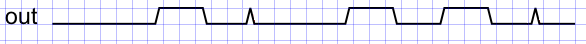
\includegraphics[width=\textwidth]{images/glitch/def_glitch_1.png}
	\caption{Zwei Glitches im Ausgangssignal}
	\label{fig.glitch.def}
\end{figure}


\section{Ursache für Glitches}\label{sect.glitch_ursache}

Der Auslöser sind ungleichzeitig eintreffende Signale, die durch

\begin{enumerate}
\item unterschiedlich lange Signalpfade,
\item unterschiedliche Durchlaufverzögerungen der vorangehenden Flip-Flops oder
\item unterschiedliche Logik-Zeiten
\end{enumerate}

entstehen, und die in ein asynchrones Bauteil geführt werden. Der Dekoder im asynchronen Bauteil entschlüsselt dadurch kurzfristig einen falschen Wert.

Abbildung \ref{fig.glitch.bild1} zeigt ein leicht verzögertes enable-Signal (ena) zu einem anders verzögerten Flip-Flop-Eingangssignal (Q). Beide Signale sind mit der Taktfrequenz clk getaktet. Der Ausgang (out) des Flip-Flops weist aufgrund der unterschiedlichen Verzögerungen kurzzeitig \textit{glitches} auf. \\
\begin{figure}[H]
	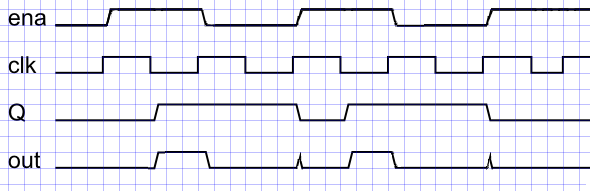
\includegraphics[width=0.8\textwidth]{images/glitch/def_glitch_3.png}
	\caption{Asynchrone Eingangssignale führen zu Glitches}
	\label{fig.glitch.bild1}
\end{figure}


\newpage
\section{Glitch erzeugen}\label{sect.glitch_detect}


\subsection{Konzept}
Glitches werden durch Pfadverlängerung einzelner Werte erzeugt. Ein asynchroner Zähler erhält verzögerte Bitwerte. Zählt man binär auf 15, so kann sich beim Übergang von der Zahl 11 zu 12, die falsche Zahl 15, ergeben, sofern die zwei höheren Bits der Zahl 11 verzögert ankommen (siehe Abbildung \ref {fig.glitch.binaer_zahlen}).

\begin{figure}[H]
	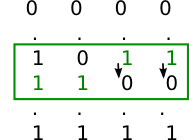
\includegraphics[width=0.3\textwidth]{images/glitch/konzept_verzoegerung.png}
	\caption{Binärwerte des asynchronen Zählers}
	\label{fig.glitch.binaer_zahlen}
\end{figure}

Die Verzögerung der zwei Bits, wird über Routing umgesetzt. 

\subsection{Implementation} 

Die Hardware ist das Altera Board De2 mit dem FPGA Cyclone II. Kompiliert wird das Projekt mit Quartus 13.0sp, der ältesten Quartus-Version, die den Cyclone II unterstützt.

Die Pfad\textit{verlängerung} wird über das Routing über die GPIO-Pins des Stecker 1 gemacht (siehe Abbildung \ref{fig.glitch.GPIO}. GPIO 1 ist der Stecker 1). Dekodiert die asynchrone Logik die Zahl 15, wird das  Reset-Signal (aus der Logik \lstinline|reset_counter\~{}2|) an den Zähler gesendet und der Zähler beginnt wieder von 0 an zu zählen. Produziert der Dekoder zur falschen Zeit einen Reset, so ist dies eine Fehlkodierung: ein \textit{glitch}.

Das RTL-Diagramm des asynchronen Zählers sieht wie folgt aus:
\begin{figure}[H]
	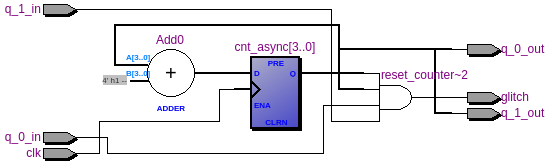
\includegraphics[width=1\textwidth]{images/glitch/RTL_asynchron.png}
	\caption{Asynchroner Zähler mit Routing erzeugt Glitch}
	\label{fig.glitch.RTL_nurGlitch}
\end{figure}

Um die Lösung gegen \textit{glitches} aufzuzeigen, wird dem asynchronen Zähler zur Synchronisation ein Flip-Flop nachgeschalten. Dadurch werden die asynchronen Zustände übersehen. 
\begin{figure}[H]
	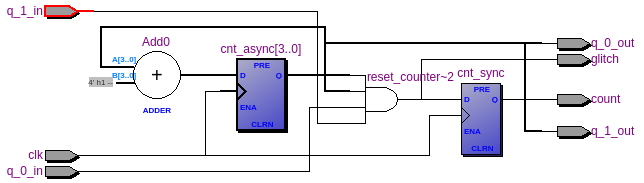
\includegraphics[width=\textwidth]{images/glitch/glitch_asynch_new.png}
	\caption{Glitch-Zähler und synchroner Zähler dazu}
	\label{fig.glitch.RTL_mit_synchr.Zaehler}
\end{figure}

Die Reset-Signale aus der Vergleichslogik (\lstinline|reset_counter\~{}2|) des asynchronen Zählers wie die des synchronisierten Zählers werden an die GPIO Steckers ausgegeben, ebenso der Systemtakt. In der Abbildung \ref{fig.glitch.GPIO}) wird das Signal des asynchronen Zählers als Glitch und das Signal des synchronisierten Zählers als Count benannt. In der GPIO-Pinbelegung sieht man auch die Nutzung der zwei oberen Pin-Reihen für das Routing (benannt mit Routing OUT, IN). Der Systemtakt wird als CLK ausgegeben.

\begin{figure}[H]
	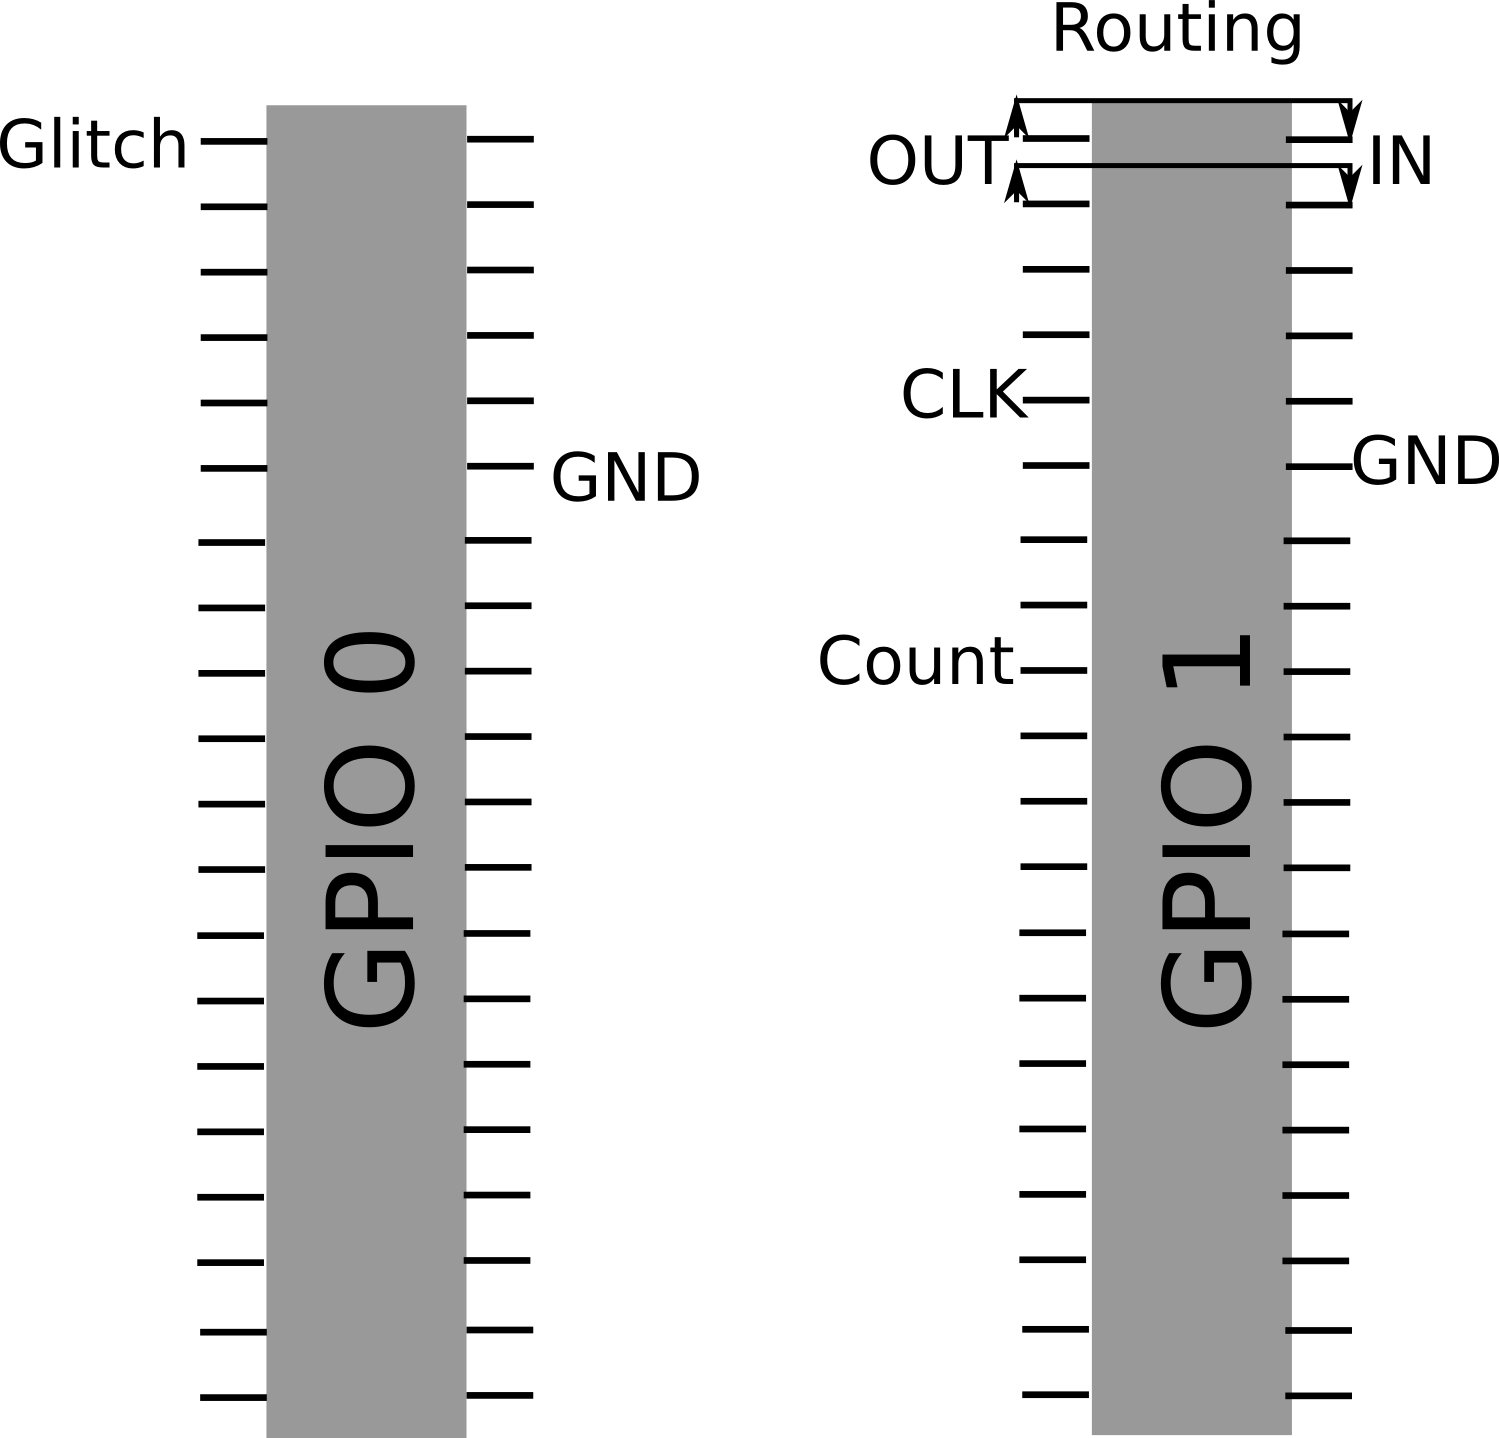
\includegraphics[width=0.5\textwidth]{images/glitch/GPIO_Belegung.png}
	\caption{GPIO Anschlüsse}
	\label{fig.glitch.GPIO}
\end{figure}


\newpage
\section{Resultat }\label{sect.glitch_resultat}

Der Reset des asynchronen Zählers (CH 1), der synchronisierte Reset (CH 2) und der Systemtakt (CH 3) werden am KO ausgegeben. Durch die Synchronisation wird der Wert um 1 Periode (= 20 ns) verzögert.

\begin{figure}[H]
	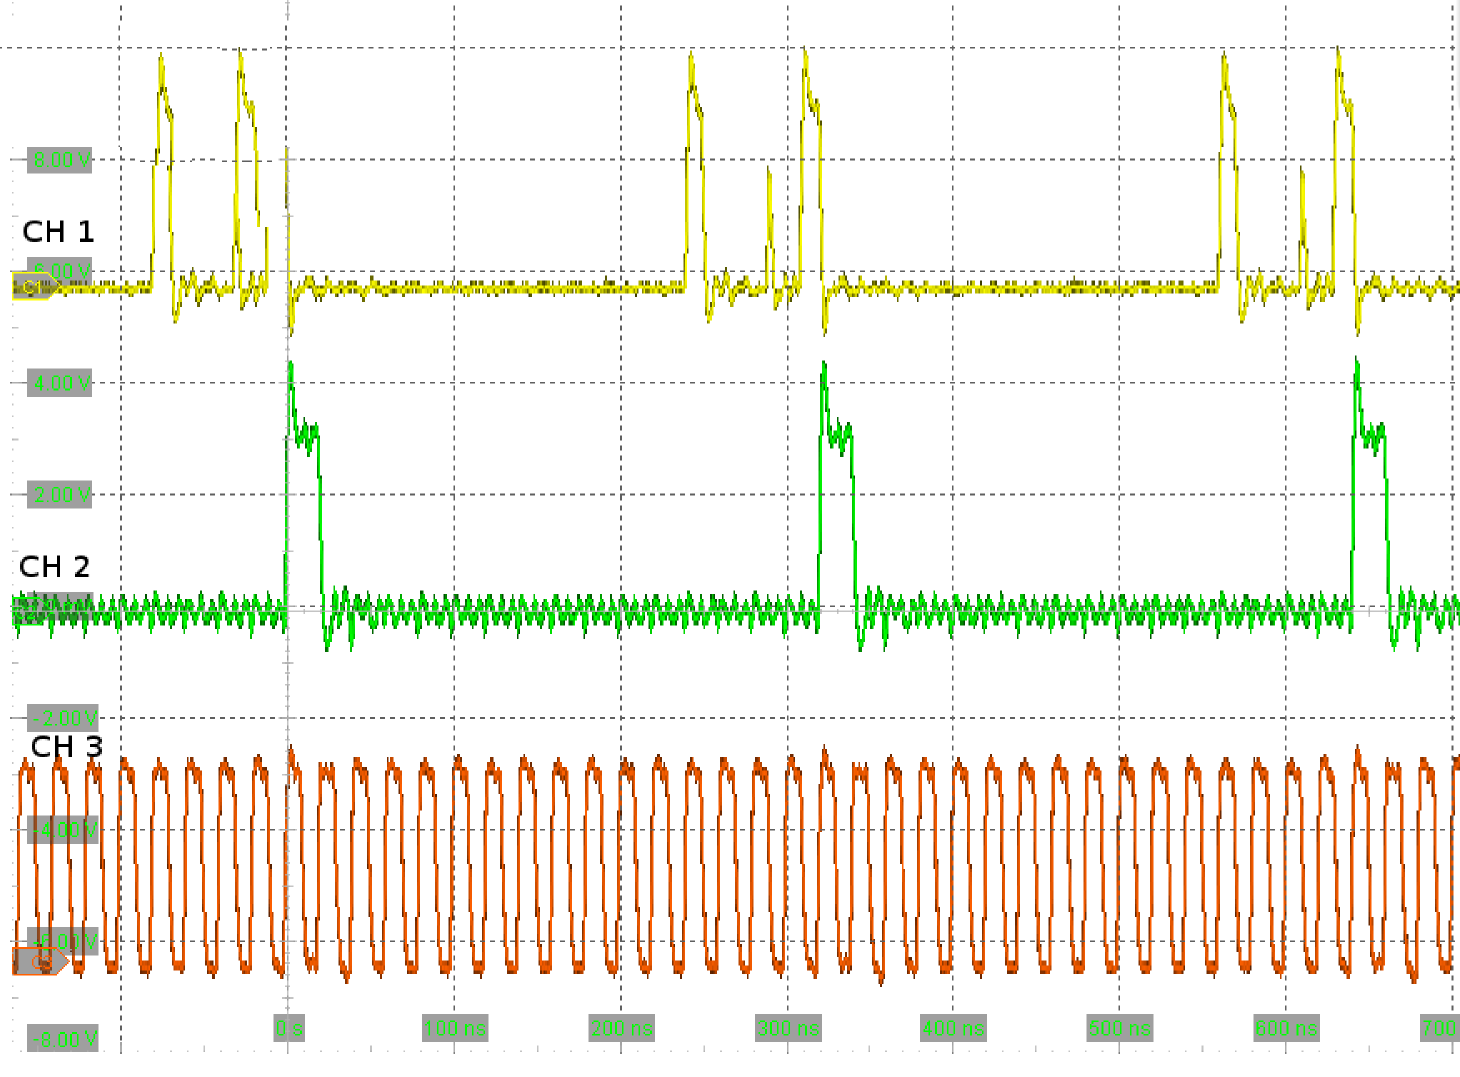
\includegraphics[width=0.6\textwidth]{images/glitch/Glitch_2_good.png}
	\caption{Glitch (gelb), Zähler (grün) und Takt (orange)}
	\label{fig.glitch.result_1}
\end{figure}

 Das \textit{glitch} trifft in der im Übergang von der 11 zur 12 Periode (nach 240 ns) regelmässig auf. Dies ist das zu erwartende Ergebnis. Ein kurzzeitiges asynchrones Verhalten findet sich auch im Übergang von der 13 zur 14 Periode. Dies ist wenn der binäre Wert 1101 auf 1110 wechselt. Da die zwei niederwertigen Bits verzögert sind, ist das Dekodieren des Wertes 1111 plausibel.\\
 
\begin{figure}[H]
	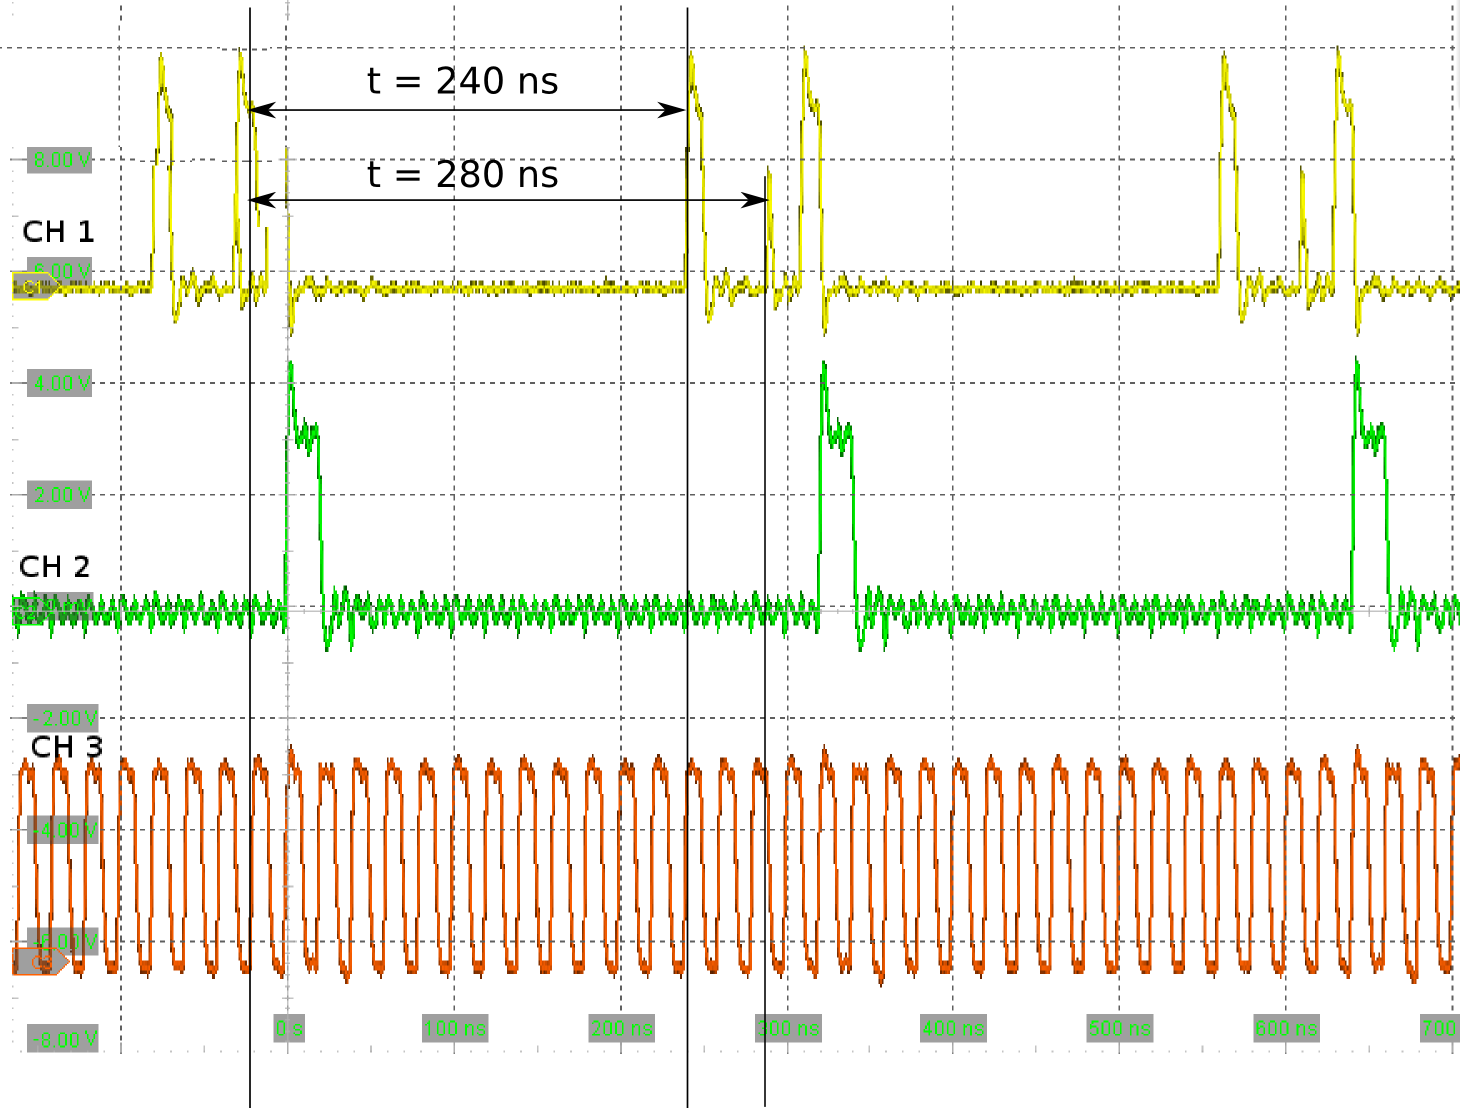
\includegraphics[width=0.6\textwidth]{images/glitch/Glitch_2_timing.png}
	\caption{Zeitanalyse Glitches}
	\label{fig.glitch.result_2}
\end{figure}



 	
	%%%%%%%%%%%%%%%%%%%%%%%%%%%%%%%%%%%%%%%%%%%%%%%%%%%%%%%%%%%%%%%%%
%  _____       ______   ____									%
% |_   _|     |  ____|/ ____|  Institute of Embedded Systems	%
%   | |  _ __ | |__  | (___    Wireless Group					%
%   | | | '_ \|  __|  \___ \   Zuercher Hochschule Winterthur	%
%  _| |_| | | | |____ ____) |  (University of Applied Sciences)	%
% |_____|_| |_|______|_____/   8401 Winterthur, Switzerland		%
%																%
%%%%%%%%%%%%%%%%%%%%%%%%%%%%%%%%%%%%%%%%%%%%%%%%%%%%%%%%%%%%%%%%%

\chapter{Metastabilität}\label{chap.metastabilitat}

\section{Definition Metastabilität}\label{sect.meatastabil_def}
Metastabilität bedeutet, dass der Ausgang eines Flip-Flops nicht dem Eingang entsprechen muss. Wechselt das Inputsignal eines Flip-Flops zur falschen Zeit, ist der Wert des Ausgangssignal unsicher. Hier zwei kurze englische Beschreibungen, dieses Phänomens:\\
\newline
'' If data inputs to a flip-flop are changing at the instant of the clock pulse, a problem known as \textit{metastability} may occur. In the metastable case, the flip-flop does not settle in to a stable state'' (Camara, S. 32-2)  \\
\newline
''If the amplitude of the runt pulse is \textit{exactly the treshold level of the SET input of the output cell}, the cell will be driven to its metastable state. The metastable state is the condition that is roughly defined as ''half SET and half RESET'' (Fletcher, 482.)\\
\newline
\\
Im besten Fall wählt der Ausgang bei unklarem Eingangssingal selbst einen Wert an ('0' oder '1'). Im schlechten Fall “hängt” sich das Flip-Flop “auf” und toggelt permanent zwischen '0' und '1' oder setzt sogar beide Werte parallel.

\begin{figure}[H]
	\centering
	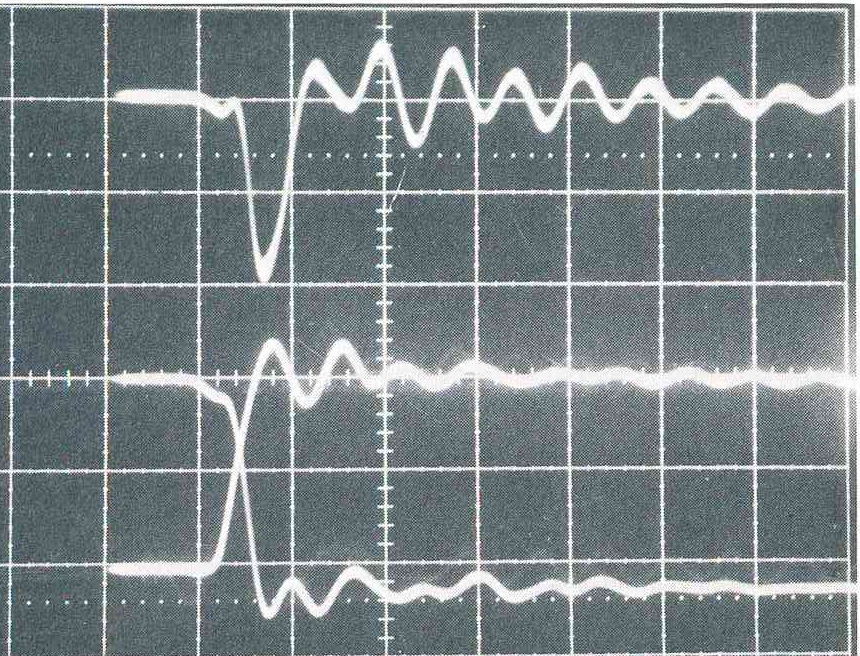
\includegraphics[width=0.4\textwidth]{images/metastability/metastability_2_IO.png}
	\caption{Metastabilität schlimmster Fall (Fletcher, 482.)}
	\label{fig.metastabil.schlimmster_Fall}
\end{figure}


\section{Ursache von Metastabilität}\label{sect.meatastabil_ursache}
Der Grund für Metastabilität ist, dass der angelgte Wert entweder zu spät eintrifft (verletzen der setup-Zeit) oder zu früh wieder verschwindet (verletzen der hold-Zeit). Metastabilität kann vermieden werden, wenn diese zwei Zeiten strikt eingehalten werden:\\
\newline
''Metastabilit is avoided by holding the information stable before and after the clock pulse  for a set period of time, called the setup time for the data line an the hold time for the control line.''(Camara, S. 32-2)
\begin{figure}[H]
	\centering
	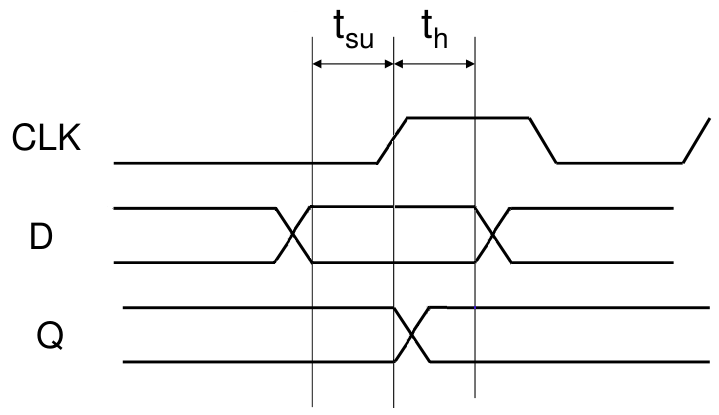
\includegraphics[width=0.4\textwidth]{images/metastability/kritscheZeit_FF.png}
	\caption{Einhalten der Datenzeiten}
	\label{fig.metastabil.kritisches_zeitfenster}
\end{figure}
Es gibt mehrere Gründe für das Nichteinhalten der geforderten setup-Zeit:\\
- Ein Logikpfad kann zu lange sein, bzw. die Taktfrequenz ist zu schnell\\
- Zwischen den Bauteilen liegen zu lange Pfade, die das Eintreffen der Daten verzögern\\
- Ein vorangehendes Bauteil hat eine zu lange Durchlaufverzögerung.\\
\\
Um Metastabilität zu vermeiden, sollte die Logik möglichst klein gehalten werden, die Bauteile bewusst nahe beieinander platziert und vor allem der Systemtakt an die längste Pfadzeit angepasst werden. Der maximal elaubte Systemtakt kann in quartus mit dem Timequest Time Analyser abgefragt werden.\\
Als Alternative bietet sich eine Synchronisierungsschaltung an. Zwischen den zwei Takt-Flanken kann sich der metastabile Ausgang erholen und gelangt so stabil in den Verarbeitungspfad. Der Nachteil der Synchronistation ist jedoch, eine um einen Takt längere Verarbeitungszeit.\\


\section{Metastabilität erzeugen}\label{sect.meatastabil_erzeugen}
\subsection{Ansatz}\label{sect.metastabil_ansatz}
Aufgebaut wird ein System mit zwei Takten. Der zentrale Block hat eine Taktfrequenz von 50 MHz und beinhaltet eine State Machine. Diese wechselt bei jedem Impuls von einem Zustand in den anderen (Abbild: \ref{fig.metastabil.statemachine} Um die zwei Zustände zu erkennen, werden beiden Zuständen ein logischer Pegel zugefügt:\\
\newline
- Zustand 1:  s0  = Logisch '0'\\
- Zustand 2:  s1  = Logisch '1'\\

\begin{figure}[H]
	\centering
	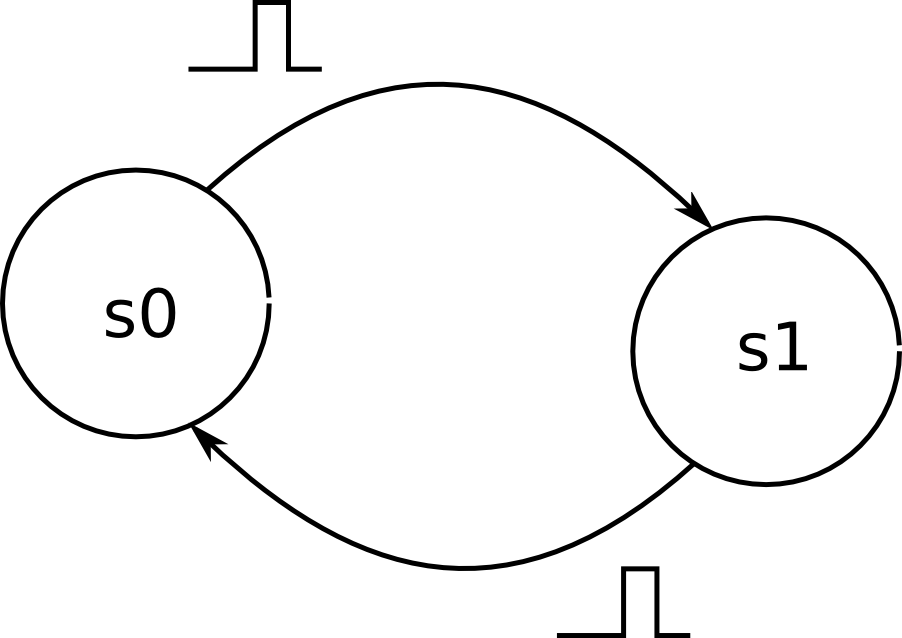
\includegraphics[width=0.2\textwidth]{images/metastability/statemachine_s0_s1.png}
	\caption{Statemachine im zentralen Block}
	\label{fig.metastabil.statemachine}
\end{figure}

Der Inpuls, der die Statemachine steuert ist asynchron. Er wird von einem Zähler generiert, der mit der Taktfrequenz von 27 MHz läuft. Alle 37 ns sendet der Zähler einen Puls an die State Machine. Die State Machine selbst arbeitet mit einer Taktfrequenz von 20 ns. Der Impuls ist ihr gegenüber asynchron.\\
\newline
Erwartet wird, dass die setup-Zeit der State Machine-Flip-Flops regelmässig verletzt werden. \\

\begin{figure}[H]
	\centering
	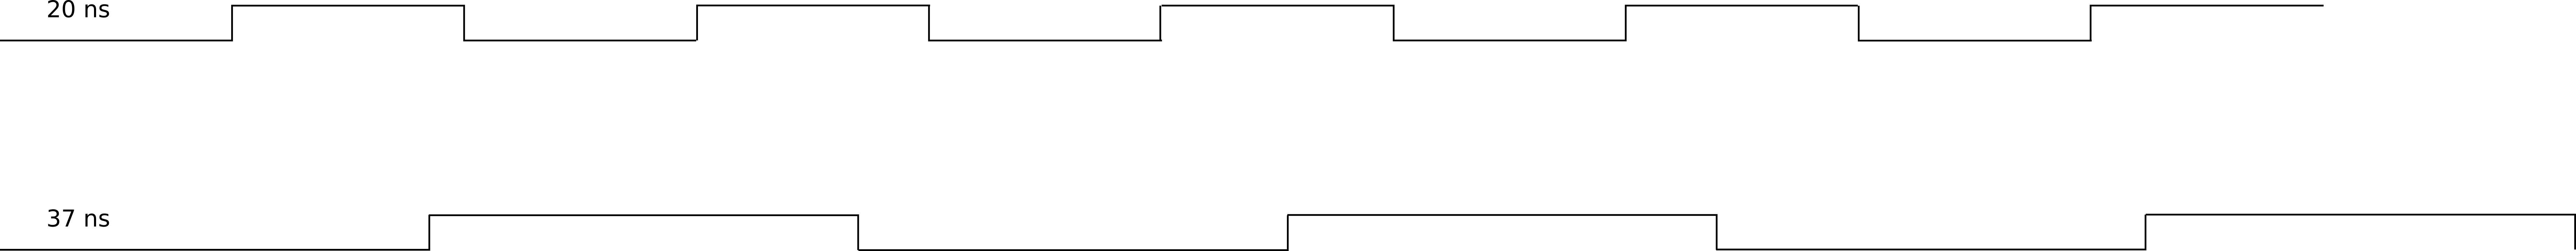
\includegraphics[width=0.2\textwidth]{images/metastability/2_takte.png}
	\caption{Die zwei Taktzeiten}
	\label{fig.metastabil.statemachine}
\end{figure}
\todo{ einsetzen setup zeit gemäss glossar für ..}


\subsection{Implementation}\label{sect.metastabil_implementation}


\section{Resultat Metastabilität provozieren}\label{sect.meatastabil_proozieren}
\textbf{Was ist das Ergebnis beim Verletzen der setup Zeit?}
Beide Ausgänge immer an?
Keiner von beiden?
aufhängen des Systems? (Keine LED geht mehr).

\textbf{Synchronisation Schaltung erhärtet die These b\\}
 
	%%%%%%%%%%%%%%%%%%%%%%%%%%%%%%%%%%%%%%%%%%%%%%%%%%%%%%%%%%%%%%%%%
%  _____       ______   ____									%
% |_   _|     |  ____|/ ____|  Institute of Embedded Systems	%
%   | |  _ __ | |__  | (___    Wireless Group					%
%   | | | '_ \|  __|  \___ \   Zuercher Hochschule Winterthur	%
%  _| |_| | | | |____ ____) |  (University of Applied Sciences)	%
% |_____|_| |_|______|_____/   8401 Winterthur, Switzerland		%
%																%
%%%%%%%%%%%%%%%%%%%%%%%%%%%%%%%%%%%%%%%%%%%%%%%%%%%%%%%%%%%%%%%%%

\chapter{Testbench}\label{chap.testen}
 \textit{Test Driven Development} bedeutet, dass vor oder parallel zur Entwicklung einer \textit{unit} (im Folgenden Block genannt) der \textit{unit test} entwickelt wird\cite{Testdriven}. Beim textbasierten Testen stammen die Befehle aus einer Input-Datei, und die Ergebnisse werden in einer Datei abgelegt. 

\section{Device Under Test}\label{sec.testbench_DUT}
Das Device Under Test (DUT) ist das MIDI Interface (siehe Abbildung \ref{fig.testbench}). Das Ziel ist, dass das MIDI-Signal in den Block geführt wird und am Ausgang 10 Notenvektoren anliegen mit je 8 Notenbits und einem Bit, das besagt, ob die Note an oder ab ist.

\begin{figure}[H]
	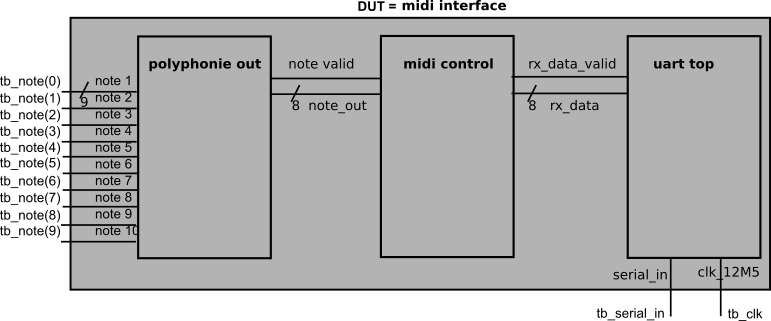
\includegraphics[width=1\textwidth]{images/midi_interface/testbench_midiinterface.png}
	\caption{Blockschaltbild Device under Test}
	\label{fig.testbench}
\end{figure} 

Die \textit{testbench} wird mit Daten der Input-Datei gespiesen. Die Endversion der Input-Datei und der Testbericht liegen im Anhang \ref{chap.anhang_midi_input}. 
In den Unterkapiteln wird der Aufbau der Input-Datei, das Entwickeln der Test-Fälle, und die Umsetzung im VHDL-Code beschrieben.


\section{Struktur der Input-Datei}\label{sec.testbench_inputdatei} 

Die Test-Datei ist zeilenweise strukturiert.

\subsubsection{Verarbeitungsmodus} 
Jede Zeile beginnt mit dem Verabreitungsmodus. Bei der Input-Datei besteht der Verarbeitungsmodus aus fünf Buchstaben.

\begin{tabbing}
\hspace{4em} \= \hspace{2em} \= \hspace{2em} \=\kill
reset	\> 00 \> 00 \> \ldots{}\\
singl	\> 90 \> 27 \> \ldots{}\\
polyp	\> 71 \> 55 \> \ldots{}
\end{tabbing}

\subsubsection{Tokenstruktur} 

Nach dem Verarbeitungsmodus folgen die Daten. Jede Zeile hat gleichviele Datenpakete (Tokens). 
Die \textit{testbench} ortet jedem MIDI-Datenpaket (siehe \ref {datentypen}, Beschreibung der MIDI-Daten) innerhalb der Zeile eine Bedeutung zu. Je nach Verarbeitungsmodus ist die Bedeutung der Token anders.

Die Tokenstruktur leitet sich aus der MIDI-Datenstruktur im \textit{polyphony mode} und im \textit{single mode} ab (siehe  \ref{note_modes}). In den nachfolgenden zwei Token-Beispielen bezieht sich die obere Zeile auf den \textit{polyphony mode} und die untere auf den \textit{single mode}.

In der \textit{testbench midi interface} haben Tokens folgende Bedeutung:


{
\renewcommand{\arraystretch}{1.0} % avoid the extra space between the rows
\begin{tabular}{@{}*{10}{l}@{}} % @{} removes the left and right margin around the table
mode\_p	& Note & Velocity	& Note & Velocity & Note & Velocity & Note & Velocity & Anzahl Noten \\
mode\_s	& Dummy & Status & Note & Status & Note & Status & Note & Dummy & Dummy
\end{tabular}
}

Dummy ist die Bezeichnung für das Einlesen nicht relevanter Werte. Diese nicht relevanten Werte sind in der Input-Datei gesetzt, um die Verarbeitungsstruktur beim Einlesen der Token zu vereinfachen. Der Dummywert wird beim Einlesen verworfen.\\
 
\section{Aufstellen der Fehler}\label{sec.testbench_fehler} 

Zu Beginn hatten die Testfälle nur drei Tokens und testeten die Grundfunktionen:\\

single mode note an/ab\\
singl 90 27\\ 
singl 90 27\\

polyphone note an/ab\\
polyp 71 55\\
polyp 71 00\\

Komplexere Testfälle zeigten, dass eine Test-Zeile mehr Tokens braucht. Die Endversion der Input-Datei kann mit einer Zeile bis 4 Noten an und abstellen.


\subsection{Einzelne Noten testen}
 
\subsubsection{Testfälle}
Getestet sind auch Kombinationen unter den Fällen, die aus Übersichtlichkeit nicht alle aufgeschrieben werden.\\
\begin{itemize}
\item Einzelne Note an, Geschwindigkeits Byte folgt
\item Einzelne Note an, Geschwindigkeits Byte folgt nicht
\item Einzelne Note ab
\item Einzelne Note an, direkt nach Reset
\item Einzelne Note an, selbe Note nochmals an
\item Einzelne Note an, wenn in \textit{polyphony mode}
\item Einzelne Note an, nach ungültigem status byte
\item Einzelne Note an, andere Note an, erste Note ab
\item Einzelne Note an, diverse andere Noten setzen, erst bei nächster Zeile erste Note ab
\end{itemize}

Zu jedem Testfall wird auf der nächsten Zeile das zu erwartende Resultat vorgegeben. Die testbench prüft die ausgegebene Notenwerte am Ausgang des MIDI interfaces mit den vorgegebenen Werten.

Beispielzeile\\
\rule{\textwidth}{0.4pt}\\
{
\renewcommand{\arraystretch}{1.0} % avoid the extra space between the rows
\begin{tabular*}{\textwidth}{@{}@{\extracolsep{\fill}}*{10}{l}@{}} % @{} removes the left and right margin around the table
singl & 55 & 90 & 27 & 80 & 27 & 90 & 05 & 00 & 00\\
check & 00 & 00 & 27 & 00 & 00 & 00 & 05 & 00 & 00\\
\end{tabular*}
}

Die Sequenz bedeutet Note 27 an (0x90), dann ab (0x80) der Note 27 und am Schluss an Note 05. \\
Überprüft (check) wird, ob am Ausgang die Noten 27 und 05 anliegen.\\
Im \textit{single mode} ist die Geschwindigkeit für das An- oder Abstellen der Note nicht relevant und wird deshalb nicht als Befehl eingelesen. Die \textit{testbench} hängt nach jeder Note einen Dummy-Geschwindigkeitswert von 0x55 an.

\subsection{Polyphonie testen }\label{polyphonitest}

\subsubsection{Testfälle}

In der Polyphony können mehrere Noten hintereinander an- und nur einzelne davon wieder abgestellt werden.

\begin{itemize}
\item Polyphoniestatus setzen, einzelne Note an
\item Polyphoniestatus setzen, mehrere Noten an
\item Polyphoniestatus setzen, mehrere Noten über mehrere Zeilen verteilt an
\item Polyphoniestatus setzen, Note an, die bereits in Register ist
\item Polyphoniestatus setzen, Note an, andere Note an, erste Note aus, dritte Note an
\item Polyphoniestatus setzen, dritte Note aus, erste Note an, erste Note an
\item Polyphoniestatus setzen, \textit{single note an} Status setzen, Note ohne Geschwindigkeit senden
\item Polyphoniestatus setzen, falsches Statusbyte senden, Note an, Note aus,
\item Polyphoniestatus setzen, Reset, Note setzen
\item Polyphoniestatus setzen, 10 Noten an
\item Polyphoniestatus setzen, 10 Noten in Register, eine ist aus. Neue Note an senden
\end{itemize}

Beispielzeile\\
\rule{\textwidth}{0.4pt}\\
{
\renewcommand{\arraystretch}{1.0} % avoid the extra space between the rows
\begin{tabular*}{\textwidth}{@{}@{\extracolsep{\fill}}*{10}{l}@{}} % @{} removes the left and right margin around the table
polyp & 71 & 55 & 02 & 55 & 33 & 55 & 08 & 00 & 00\\
check & 71 & 00 & 02 & 00 & 33 & 00 & 00 & 00 & 03
\end{tabular*}
}

In der Sequenz wird die Note 71, dann die Noten 02 und 33. Danach wird die Note 08 abgestellt. Die \textit{testbench} prüft am Ausgang, ob die Noten 71, 02 und 33 an sind. 

Im Verarbeitungsmodus Polyphonie sendet die \textit{testbench}  das \textit{status byte} "10100000" (0xA0) 



\section{Code Testbench}\label{sec.code_testbench}

Die automatisierte Datenverarbeitung erzeugt viele Werte (10 Noten mit je 9 Werten). Um einzelne Bits effizient zu setzen oder zu überprüfen, wird der Code einem \textit{refactoring} unterzogen.

Im Gegensatz zum hardwarenahen Code der VHDL-Blocks, bei denen arrays und loop explizit vermieden wurden, baute die \textit{testbench} bewusst auf softwarenahe Strukturen auf.

\subsection{Package}

Damit in allen VHDL-Dateien die Arrays und Konstanten gebraucht werden können, werden diese Definitionen in einem Package zusammengefasst. Das Package kann wie eine Library zu Beginn einer VHDL-Datei eingebaut werden.
\begin{itemize}
	\item Werte der \textit{status bytes} als Konstanten
	\item Ein- und Ausgänge als arrays
	\item Tokenstruktur als record
\end{itemize}

Bsp. Tokenstruktur

\begin{lstlisting}[language=vhdl]
-- define midi_data
type t_midi_data is record
    token_note : std_logic_vector(7 downto 0);
    token_attribut : std_logic_vector(7 downto 0);
    end record;

type t_midi_data_array is array (0 to 3) of t_midi_data;

-- define token structure
type t_token_line is record
    token_cmd : string(1 to 5);
    t_midi_data : t_midi_data_array;
    token_number : std_logic_vector(7 downto 0);
    end record;

-- array with note structure (input/output)
type t_note_array is array (0 to 9) of std_logic_vector(8 downto 0);
\end{lstlisting}


\subsection{Prozess-Optimierung}

Um die einzelnen Bits in den arrays zu setzen, braucht es in der Ablaufstruktur Optimierungen.

\begin{itemize}
	\item Loops iterieren durch die arrays
	\item Einleseprozess wird vom Verarbeitungsprozess getrennt
	\item Flags wie \lstinline|s_read_input_finished <= '1'| sichern das parallele Datenverarbeiten
\end{itemize}

\section{Ergebnisse Simulation}\label{sec.ergebnisse_tests}
Die Ausgabe der Signale in die Output-Datei bezieht sich auf den Zustand am Ausgang des DUT. Damit auch die beiden internen Blöcke MIDI control und Polyphonie out korrekt funktionieren werden die Signale überprüft. Auch das Verhalten in den Blöcken entspricht den erwarteten Signalverläufen.

\subsection{Block Midi Control}

Gemäss der \textit{fsm} durchläuft der \textit{single mode}  die Zustände \lstinline|idle|, \lstinline|note_s|, \lstinline|velocity_s| und geht dann zurück  in den Idle-Zustand. Das Signal \lstinline|s_note_on| wechselt nach einem \textit{status byte} von (0x90) auf on und nach (0x80) auf ab.

\begin{figure}[H]
	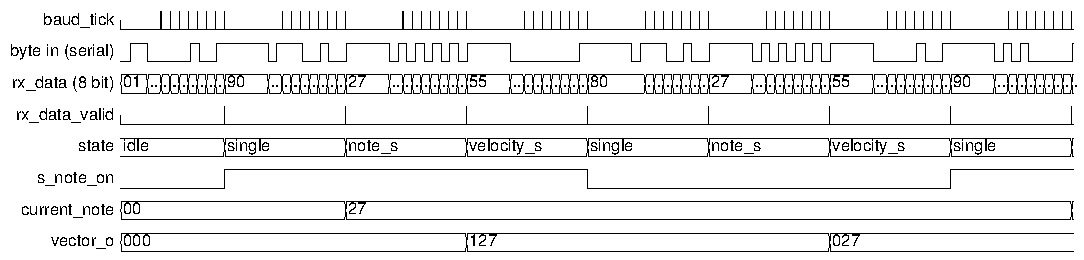
\includegraphics[width=1\textwidth]{images/midi_control/wave_single.png}
	\caption{Simulation Block Midi Control}
	\label{fig.test_midi:control_single}
\end{figure} 

Im \textit{polyphony mode} existieren die Zustände \lstinline|idle|, \lstinline|note_v|, \lstinline|velocity_v| und verbleibt in diesem Zustand. Nur durch ein \textit{status byte} (oder ungültige \textit{data bytes}) wird der Zustand der Polyphonie verlassen.

\begin{figure}[H]
	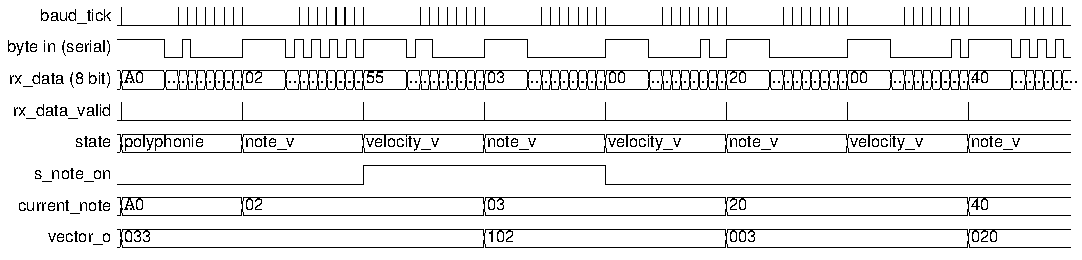
\includegraphics[width=1\textwidth]{images/midi_control/wave_polyphonie.png}
	\caption{Simulation Block Midi Control}
	\label{fig.test_midi:control}
\end{figure} 

\subsection{Block Polyphony Out}

Kriterien in der Polyphonie out sind, dass jede neue Note auf den nächsten freien Register-Platz gelegt wird. Zudem soll keine Note zwei Registerplätze belegen. Zudem soll, wenn alle Register-Plätze einen Notenwert haben, die neue Note an einen Registerplatz mit aktuell abgeschalteter Note besetzen.\\
Alle Kriterien (siehe \ref {test_polypohnie}) sind erfüllt.

\begin{figure}[H]
	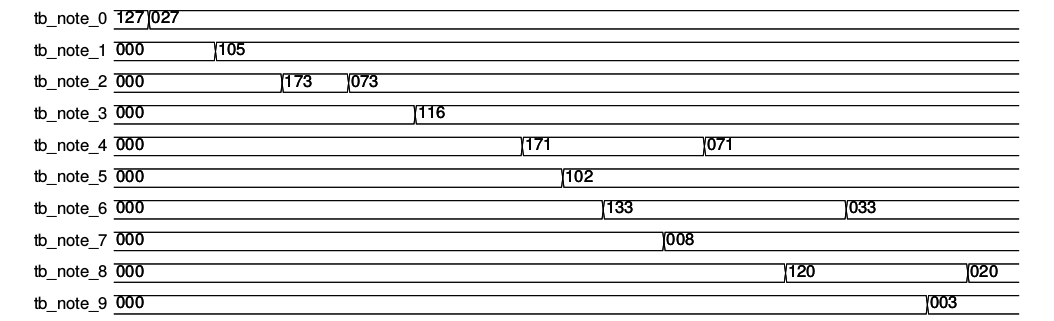
\includegraphics[width=1\textwidth]{images/midi_interface/tb_polyphonie.png}
	\caption{Simulation Block Polyphony Out}
	\label{fig.test_polyphonie}
\end{figure} 
 
	%%%%%%%%%%%%%%%%%%%%%%%%%%%%%%%%%%%%%%%%%%%%%%%%%%%%%%%%%%%%%%%%%
%  _____       ______   ____									%
% |_   _|     |  ____|/ ____|  Institute of Embedded Systems	%
%   | |  _ __ | |__  | (___    Wireless Group					%
%   | | | '_ \|  __|  \___ \   Zuercher Hochschule Winterthur	%
%  _| |_| | | | |____ ____) |  (University of Applied Sciences)	%
% |_____|_| |_|______|_____/   8401 Winterthur, Switzerland		%
%																%
%%%%%%%%%%%%%%%%%%%%%%%%%%%%%%%%%%%%%%%%%%%%%%%%%%%%%%%%%%%%%%%%%

\chapter{MIDI Steuerung}\label{chap.midi}

\section{Einteilen der Blöcke und definieren der Schnittstelen}

Als erstes die Zusammenfassung der internen Blöcke. Die zwei entwickelten Blöcke \textbf{midi control} und \textbf{polyphonie out} sind grau markiert (siehe Abbildung \ref{fig.midi_interface_block} ). Gegeben ist der Block uart top. \\

\begin{figure}[H]
	\centering
	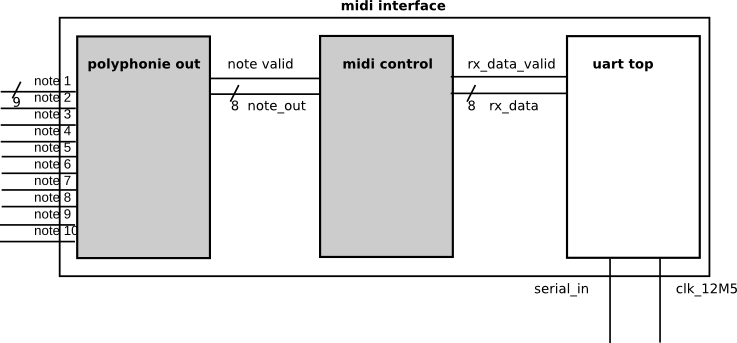
\includegraphics[width=1\textwidth]{images/midi_interface/midi_interface_block.png}
	\caption{Blockschaltbild MIDI Interface}
	\label{fig.midi_interface_block}
\end{figure}

Die Abbildung \ref{fig.top_synthesizer_block} (im Anhang \ref{chap.anhang_top_synthesizer}) zeigt, wie das zu entwickelnde MIDI Interface in die bestehenden Blöcke des Synthesizer-Projektes eingebaut wird. Die im Anhang direkt anschliessende Abbildung \ref{fig.top_synthesizer_detail} zeigt dann die geplante Umsetzung detaillierter.\\




Als nächstes wird die MIDI 1.0 Spezifikation, erklärt, nach der Block \textit{midi control} aufgebaut ist. Die Umsetzung des \textit{polyphone out}-Blocks bildet den Abschluss dieses Kapitels.\\


\newpage
\section{Das MIDI Kommunikationsprotokoll}\label{sect.midi_spezification}
Werden MIDI Daten übermittelt, so unterscheidet der Standard zwei Typen an Daten \ref{Midi_specification}.

\subsection{MIDI Daten Typen}\label{datenytpen}
\subsubsection*{Status Bytes}
\textit{Status bytes} sind 8 Bit lang und das MSB ist immer logisch '1'.  \textit{Status bytes} dienen dem Identifizerein der nachfolgenden \textit{data bytes}. Das \textit{status byte} definiert die Datenstruktur der folgenden \textit{data bytes}.
\newline
\newline
MIDI behält einen Status, bis ein neues \textit{status byte} folgt. Dieses Verhalten ist als \textit{running status} bezeichnet. Dieses Verhalten ist für Polyphonie relevant, da der Zustand bleibt, bis dass ein neues \textit{status byte} folgt..

\subsubsection*{Data Bytes}
Gemäss Spezifikation folgen einem \textit{status byte} exakt ein oder zwei Bytes. Das MSB ist immer logisch '0'. Die Werte können von 0x00 bis 0x7F sein. Das bedeutet, dass MIDI maximal 128 Noten unterscheiden kann.
\newline
\newline
\textit{Data bytes} können unterschiedliche Informationen erhalten. Im Kontroller sind Notenwerte, Geschwindigkeit des Anschalges relevant
\newline
\newline
Je nachdem \textit{status byte} werden die \textit{data byte} anders interpretiert. 
\newline
\newline
''Empfänger sollen so konzipiert sein, dass zuerst alle\textit{data bytes} empfangen werden und ein neues \textit{status byte} kommt. Danach werden ungültige Daten verworfen. Einzige Ausnahme ist der \textit{running status}. Bei dem nicht bis zum Ende gewartet wird.''\ref{Midi_specification}.\\

\subsubsection*{Ungültige Bytes}
''Alle \textit{status bytes}, die nicht implementierte Funktionen enthalten und alle ihnen folgenden \textit{Data Byte}s sollen vom Empfänger verworfen werden.''\ref{Midi_specification}.\\ MIDI Geräte sollen ausdrücklich beim Ein- und Abstellen darauf bedacht sein, dass keine undefinierten Bytes gesendet werden\ref{Midi_specification}.\\
Diese Anforderung ist wichtig beim Implementieren der \textit{finate state machine} und der \textit{testbench} (siehe \ref{polyphonitest}) \\

\subsubsection*{Midi Bytes binär}\label{midi_binaer}
\begin{itemize}
	\item ''0xxx xxxx'': \hspace*{10mm}Definition \textit{data byte}
	\item ''1xxx xxxx'': \hspace*{10mm}Definition \textit{status byte}		
	\item ''1000 xxxx'': \hspace*{10mm}Definition NOTE OFF
	\item ''1001 xxxx'': \hspace*{10mm}Definition NOTE ON
	\item ''1010 xxxx'': \hspace*{10mm}Definition POLYPHONY
	\item ''100x xxx'' \hspace*{11mm}Erste drei Bits der \textit{status bytes} NOTE ON (0x90) und NOTE OFF (0x80)
\end{itemize}
%---5.2-----------------------------------------------------------------------
\newpage
\subsection{Zwei MIDI-Noten-Modi}\label{note_modes}
\subsubsection{Datenstruktur}
Die Datenstruktur der zwei MIDI-Noten-Modi beginnt mit dem \textit{status byte} (grau in der Abbildung \ref{fig.testbench_single_Mode}). Es folgt der Notenwert (hier einen Dummy-Wert von 0x11 eingetragen) und die Geschwindigkeit. Letztere hat im \textit{single mode} keine spezfiische Bedeutung, im \textit{polyphony mode} bestimmt die Geschwindigkeit, ob die Note an oder ab ist.\\


\begin{figure}[H]
	\centering
	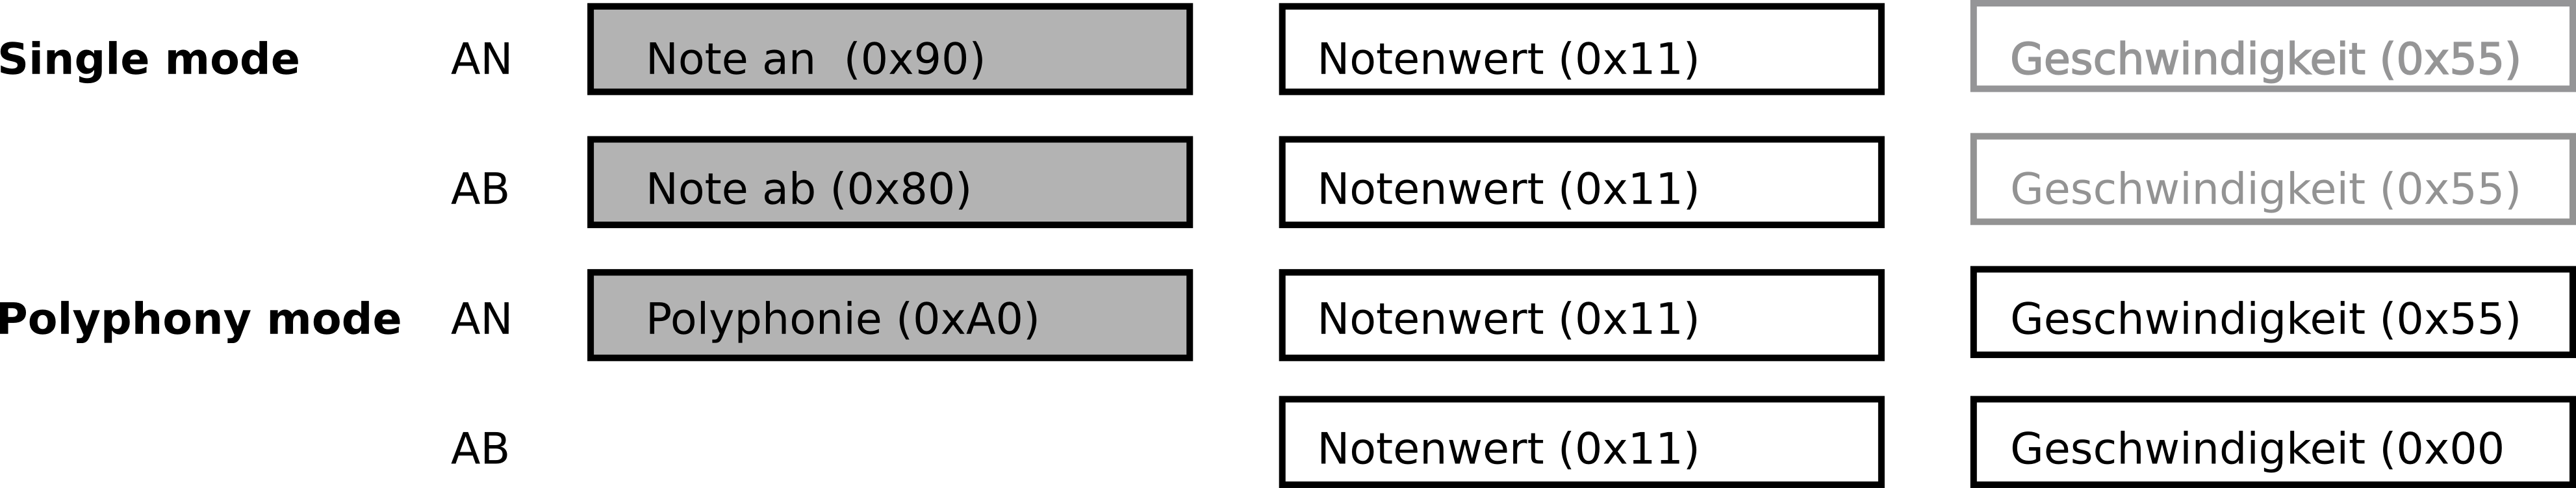
\includegraphics[width=1\textwidth]{images/midi_interface/MIDI_Spezifikation.png}
	\caption{MIDI Spezifikation für Datenstruktur einzelne Note und Polyphonie}
	\label{fig.testbench_single_Mode}
\end{figure}

Unterschiedlich zu behandeln ist die Funktion des \textit{status bytes}. Im \textit{single mode} wird mit dem \textit{status byte} der Zustand an oder ab mitgegeben. Im \textit{polyphony mode} wird nur der Noten-Modus mitgeteilt und das \textit{status byte} hat keine weiteren Funktionalitäten. In der Abbildung wird der Platz von Note an oder ab bezüglich dem Noten-Byte durch graue Markierung veranschaulicht. Die zeitliche Reihenfolge der ist umgekehrt, was in der Token-Verarbeitung berücksichtigt werden muss.\\

\begin{figure}[H]
	\centering
	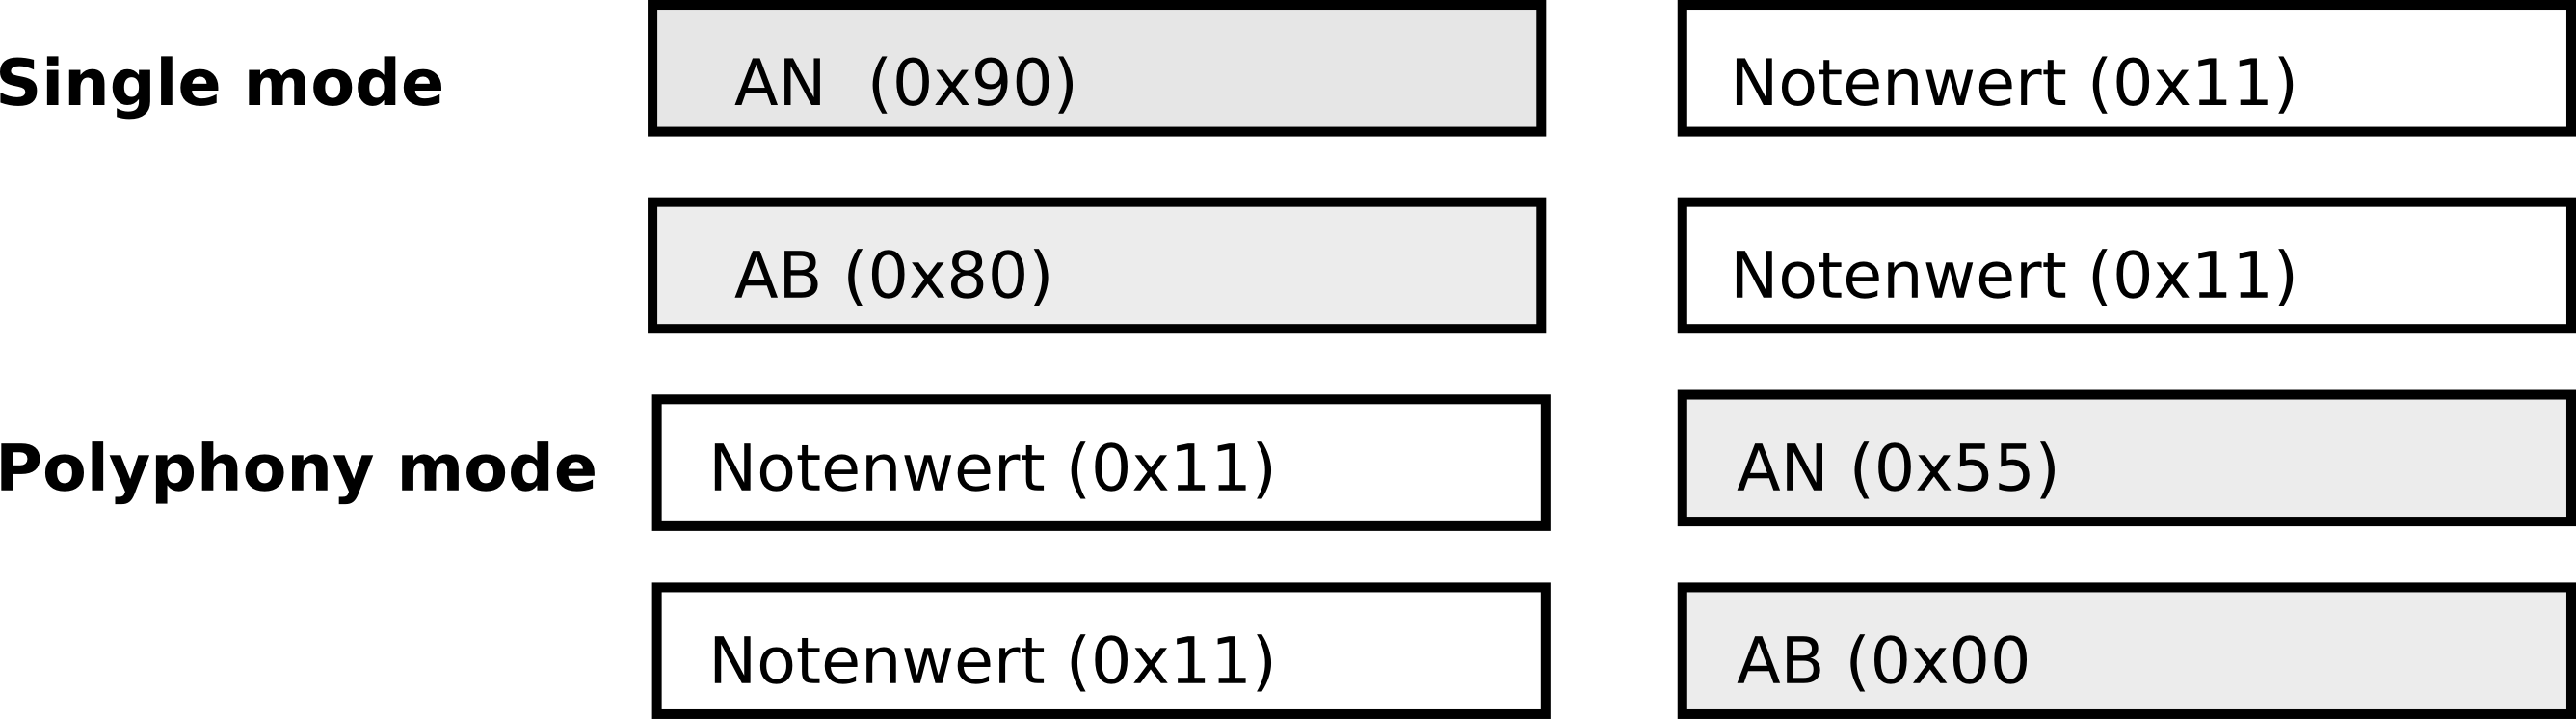
\includegraphics[width=0.7\textwidth]{images/midi_interface/MIDI_Spezifikation_Datenfolge.png}
	\caption{Blockschaltbild Device under Test}
	\label{fig.testbench_polypphon_mode}
\end{figure}

Wegen der unterschiedlichen Bedeutung der eingegangenen Token, behandelt die \textit{fsm} die zwei Noten-Modi und deren Noten- und Geschwindigkeitszustände unabhängig voneinander.



%------5.3-------------------------------------------------------------
\newpage
\section{Umsetzung Midi Control-Block}\label{sect.midi_umsetzung}

\subsection{Anforderung an die Finate State Machine und Skizze}\label{anforderung_fsm}
Der Controller wird über eine \textit{finite state machine} implementiert. Ausgehend von der Spezifikation \ref{sect.midi_spezification} sind drei Eckpunkte berücksichtigt:
\begin{enumerate}
	\item Unterscheiden von \textit{status byte} und \textit{data byte}
	\item Unterschiedliche Interpretation der \textit{data bytes} abhängig vom \textit{status byte}.
	\item Verwerfen aller falschen \textit{status byte} oder \textit{data bytes}
\end{enumerate}
\smallskip
Vereinfacht verhält sich die \textit{fsm} wie in Abbildung \ref{fig.midi_fsm_skizze} gezeigt. 
\begin{figure}[H]
	\centering
	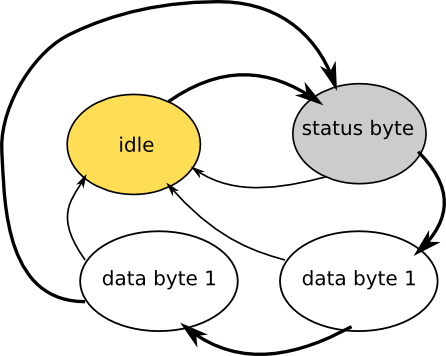
\includegraphics[width=0.3\textwidth]{images/midi_control/fsm_grob_2.png}
	\caption{Skizze der fsm}
	\label{fig.midi_fsm_skizze}
\end{figure}

Startpunkt der Verarbeitung ist das \textit{status byte} (grau hinterlegt). Danach führt die Verarbeitung durch die zwei \textit{data bytes}. \\
In jedem Zustand, werden ungültige Daten verworfen, und führen zurück zu idle. Die Verarbeitung wird fortgesetzt, wenn das nächste \textit{status byt}e folgt.\\
\newline
Nicht angeschrieben sind die Übergangsbedingungen: data\_valid = '1' wechselt zwischen den Zustänen und data\_valid = '0' verbleibt im Zustand. Die breiteren Pfeile heben die fehlerfreie Datenverarbeitung hervor.\\

\subsection{Implementation Finate State Machine}
Aufgrund der unterschiedlichen Datenstruktur für den \textit{polyphony mode} und den \textit{single mode} besitzen beide Noten-Modi ihre eigenen Zustände (siehe Abbildung \ref{fig.midi_fsm_detail}). \\ 
\newline
Die implementierten Zustände sind
\begin{itemize}
	\item idle: \hspace*{19mm}Alle nicht näher spezifizierten Vorfälle verwerfen
	\item single: \hspace*{16mm}Eintreten in  \textit{single mode} durch \textit{status bytes} 0x80 oder 0x90
	\item note\_s: \hspace*{15mm}Erstes \textit{data byte} im  \textit{single mode}
	\item velocity\_s: \hspace*{10mm}Zweites \textit{data byte} im \textit{single mode}
	\item polyphonie: \hspace*{8mm}Eintreten in polyphony mode durch status byte 0xA0
	\item note\_v:  \hspace*{15mm}Erstes \textit{data byte} im  \textit{polyphony mode}
	\item velocity\_v:  \hspace*{10mm}Zweites \textit{data byte} im  \textit{polyphony mode}
\end{itemize}


\newpage
Abbildung \ref{fig.midi_fsm_detail} definiert die Übergangsbedingungen. Drei generelle Verhaltensweisen sind vereinfacht angegeben:

\begin{itemize}
	\item data\_valid = '0'\hspace*{10mm}Im akutellen Zustand bleiben.\\
	 \hspace*{34mm}Dargestellt mit Pfeil an Ort
	\item data\_valid = '1'\hspace*{10mm}Grundbedingung für Zustandswechsel\\
	\hspace*{34mm}Gilt implizit zu jedem Pfeil und dessen Bedingung dazu
	\item data(7) = '1' and (data(7 downto 5) /=''100'' or data(7 downto 4)/= ''1010'') \hspace*{5mm} \\
	\hspace*{34mm}\textit{Status bytes}, die nicht \textit{polyphony} oder \textit{single mode} bedeuten, verworfen\\
	\hspace*{34mm}Dargestellt durch Pfeil oben rechts zu idle. Gilt für jeden Zustand
\end{itemize}
\bigskip

Die Übergangsbedingungen detektiert die Binärstruktur der MIDI Daten, die im Unterkapitel \ref{midi_binaer} aufgelistet ist.


\begin{figure}[H]
	\centering
	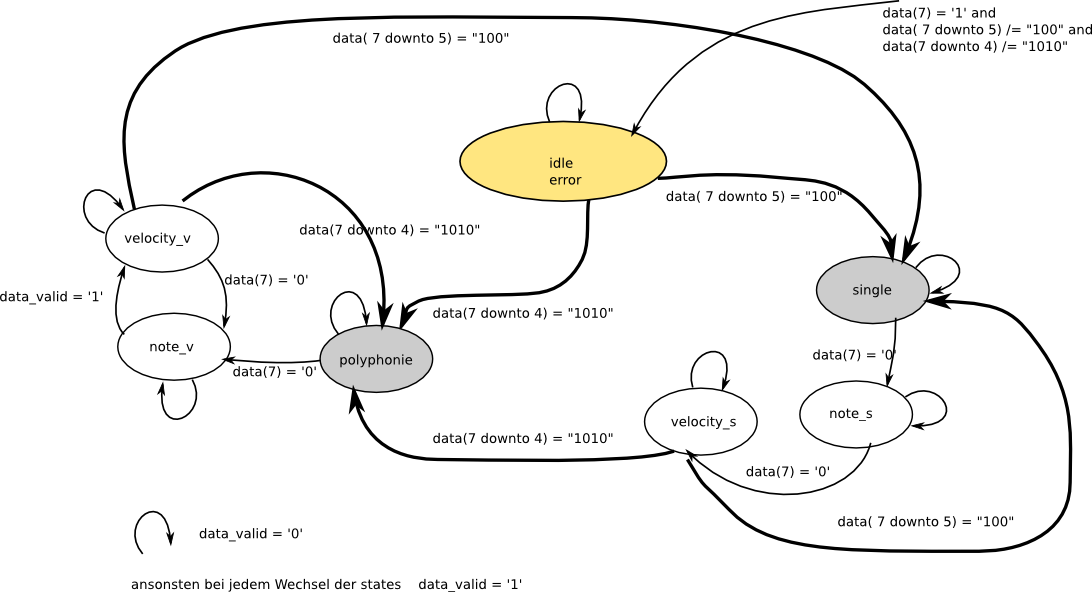
\includegraphics[width=1\textwidth]{images/midi_control/fsm_detailliert.png}
	\caption{Übergänge der fsm}
	\label{fig.midi_fsm_detail}
\end{figure}

Alle drei Anforderungen \ref{anforderung_fsm}, die sich aus der Midi Spezifkation ergeben, sind implementiert:
\begin{enumerate}
	\item Vor jedem \textit{data byte} muss ein \textit{status byte} eingegangen sein. Die \textit{finite state machine} fragt im \textit{idle} Zustand nur nach den \textit{status bytes}. Nach dem \textit{status bytes} erwartet die \textit{finate state machine} \textit{data bytes}. 
	\item Die unterschiedliche Datenstruktur der zwei Noten-Modi ist mode-spefifisch implementiert:\\
Im \textit{single mode} wird das vierte Bit des \textit{status bytes} zum Setzen von an und ab verwendet . \\
Im \textit{polyphony mode} wird das zweite \textit{data byte}, die Geschwindigkeit zum Setzen der Note auf an oder ab verwendet. \\ Geschwindigkeit = NULL ist als Note aus implementiert.\\
	\item Ungültige Bytes sind verworfen, und die \textit{fsm }kehrt in den   \textit{idle} Zustand zurück.
\end{enumerate}


%------5.4------------------------------------------------------------
\newpage
\section{Resultat Midi Control-Block}\label{sect.midi_resultat}

\subsection{Implementierte Finate State Machine}
Das ist die in quartus generierte \textit{fsm} des Blocks \textit{midi control}.
\begin{figure}[H]
	\centering
	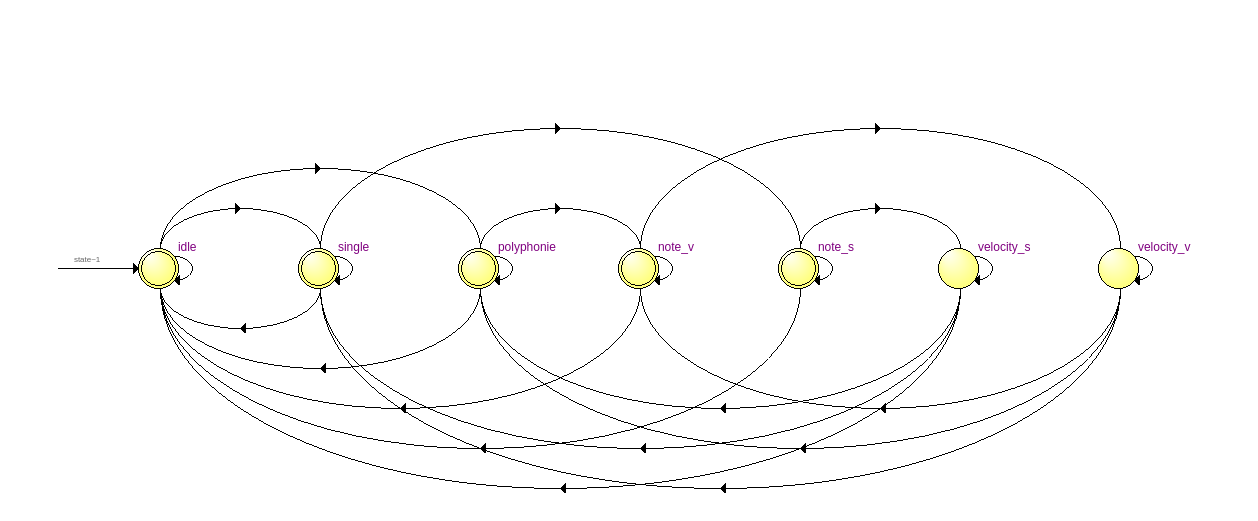
\includegraphics[width=1\textwidth]{images/midi_control/fsm_midicontrol.png}
	\caption{Implementierte fsm im Block Midi Control}
	\label{fig.midi_fsm_quartus_}
\end{figure}


\subsection{Simulation Single Mode}

\textbf{Input Daten} (Zeile 3, siehe Anhang \ref{chap.anhang_midi_input})\\
55 90 27 80 27 90 02 00 00

\textbf{Beschreibung der Befehle}\\
- 55 als Dummy-Velocity für alle Noten\\
- Note an\\
- Notenwert 27\\
- Note ab\\
- Notenwert 27\\
- Note an\\
- Notenwert 02\\
- Dummywerte\\

\textbf{Erwartetes Resultat}\\
Der Kontroller erkennt die Note 27, schaltet diese an und gibt am Ausgang den Vektor ''Note-27-AN'' aus. Dieselbe Note wird nochmals detektiert, diesmal als ab und der Vektor am Ausgang zeigt ''Note-27-AB'' an. Die nächste Note hat den Wert 2 und wird auf AN gesetzt. Der Ausgang gibt ''Note-2-AN'' aus.\\


\newpage

\begin{figure}[H]
	\centering
	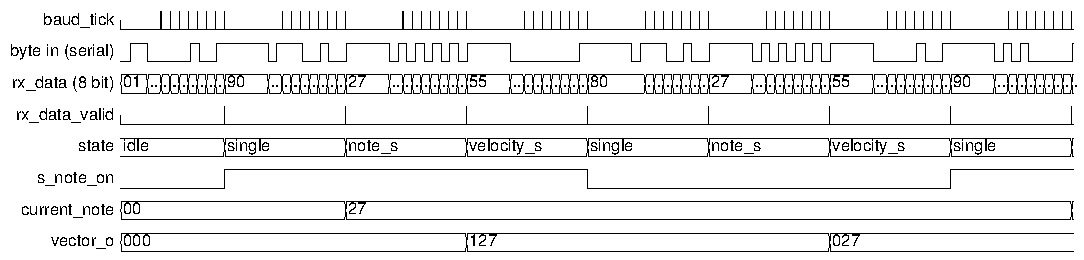
\includegraphics[width=1\textwidth]{images/midi_control/wave_single.png}
	\caption{fsm für single mode}
	\label{fig.midicontrol_singlet}
\end{figure}

\begin{itemize}
	\item Das Signal rx\_data detektiert die Befehle (0x90) und (0x80).
	\item Der Controller interpretiert  \textit{single modus}. 
	\item Die Zustandsabfolge ist korrekt: single, note\_s, velocity\_s.
	\item Zustände werden bei rx\_data\_valid = '1' die Zustände geändert.
\end{itemize}

Die Simulation zeigt, dass die Notenwerte korrekt gespeichert sind und dass das An- und Abstellen der Noten funktioniert. Am Ausgang erscheint der zusammengesetzer Vektor aus den 8 Notenbits und einem vorangestellten Bit, das detektiert, ob die aktuelle Note an oder ab ist. 



\subsection{Simulation Polyphony Mode}
\textbf{Input Daten} (Zeile 11, siehe Anhang \ref{chap.anhang_midi_input})\\
02 55 03 00 20 00 40 55 00

\textbf{Beschreibung der Befehle}\\
- Notenwert 02\\
- Note an\\
- Notenwert 03\\
- Note ab\\
- Notenwert 02\\
- Note ab\\
- Notenwert 40\\
- Note an\\

\textbf{Erwartetes Resultat}\\
Der Kontroller erkennt die Note 02, schaltet diese an und gibt am Ausgang den Vektor ''Note-02-AN'' aus. Die Note 03 wird detektiert, auf ab gesetzt und der Vektor am Ausgang zeigt ''Note-03-AB'' aus. Die nächste Note hat den Wert 2 und wird auf ab gesetzt. Der Ausgang gibt ''Note-2-Ab'' aus. Als letztes folgt die Note 40, die angestellt wird.\\

\begin{figure}[H]
	\centering
	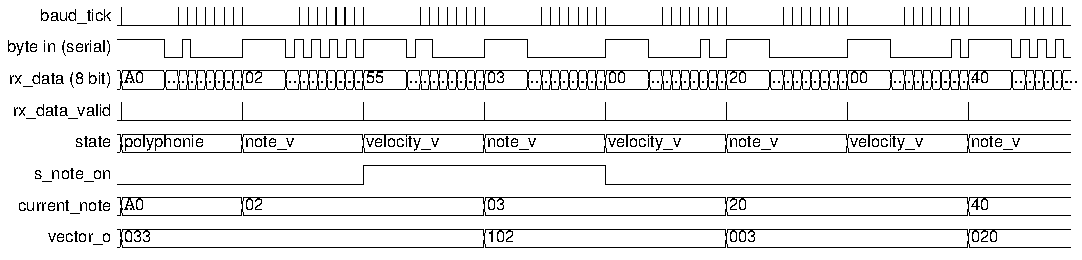
\includegraphics[width=1\textwidth]{images/midi_control/wave_polyphonie.png}
	\caption{fsm im polyphony mode}
	\label{fig.midicontrol_polyphonie}
\end{figure}


\begin{itemize}
	\item Das Signal rx\_data detektiert den Befehle (0xA0).
	\item Der Controller interpretiert  \textit{polyphony mode}. 
	\item Die Zustandsabfolge ist korrekt: polyphonie, note\_v, velocity\_v.
	\item Der Controller wartet mit dem Setzen der Note am Ausgang, bis klar ist, ob die Note an oder ab ist. \\
	Keine kurzfristig falschen Noten am Ausgang, die ab sind.
	\item Zustände werden bei rx\_data\_valid = '1' die Zustände geändert.
	\item Noten können beliebig an- und abgestellt werden
\end{itemize}


\section{Umsetzung "polyphonie out"-Block}\label{sect.polyphonie_umsetzung} 	
	%%%%%%%%%%%%%%%%%%%%%%%%%%%%%%%%%%%%%%%%%%%%%%%%%%%%%%%%%%%%%%%%%
%  _____       ______   ____									%
% |_   _|     |  ____|/ ____|  Institute of Embedded Systems	%
%   | |  _ __ | |__  | (___    Wireless Group					%
%   | | | '_ \|  __|  \___ \   Zuercher Hochschule Winterthur	%
%  _| |_| | | | |____ ____) |  (University of Applied Sciences)	%
% |_____|_| |_|______|_____/   8401 Winterthur, Switzerland		%
%																%
%%%%%%%%%%%%%%%%%%%%%%%%%%%%%%%%%%%%%%%%%%%%%%%%%%%%%%%%%%%%%%%%%

\chapter{Diskussion und Ausblick}\label{chap.diskussion}

Das Provozieren von \textit{glitch} und von \textit{metastability} ist vollständig umgesetzt. Für die entwickelte MIDI-Schnittstelle fehlt die Integration des Blocks ins Synthesizer-Projekt. 

\section{Einbauen in das bestehende Synthesizer-Projekt}

Die Schnittstellen für die Integration sind definiert (siehe Anhang \ref{chap.anhang_top_synthesizer}). Zwischen der MIDI-Schnittstelle und dem Audio Codec wird ein Tone-Generator-Block eingebaut. Der Tone-Generator beinhaltet 3 Block-Einheiten, von denen zwei bereits im Synthesizer-Projekt aufgebaut sind: Einen Tone-Dekoder-Block (bestehend), einen FM-Synthesizer-Block (bestehend) und einen Mixer (neu). Letzterer muss aufgesetzt werden, da von den ersten zwei Block-Kategorien jeweils 10 Instanzen eingebaut werden (siehe Abbildung \ref{fig.top_synthesizer_detail}). 

Bereits umgebaut ist der Tone-Dekoder. Zur ursprünglichen Auswahl, dass 12 Töne über die Schalter eingestellt werden können, werden neu 127 dekodiert. Der FPGA-Schalter 13 dient zur Auswahl, ob man die Töne vom Keyboard (Schalter auf logisch '1') oder wie bisher von den restlichen 12 Schaltern auslösen will.\\
Bereits implementiert ist die 10-fache Instanzierung der Ton-Dekoder und die 10-fache Ausführung des bestehenden FM-Synthese-Blocks. Die Instanzen sind ins Top-Level eingebaut und verbunden (siehe Abbildung \ref{fig.rtl_top_synthesizer}). Die Ausgänge der 10 FM-Synthese-Blöcke führen auf einen Mixer. Von diesem besteht das Grundgerüst und ein erster Ansatz, die 10 Signale über Addition zu einem Signal zusammen zu führen. Dieser Ansatz ist nicht ausgereift und muss überprüft werden.

Da der Mixer die Signale nicht zu einem vereinen konnte, konnte kein polyphones Signal an den Audio-Codec übertragen werden. 

\section{Frequenzmodulation mit vielfältiger Klangfarbe}

Was nicht implementiert ist, ist eine anspruchsvollere Frequenzmodulation mit vielfältiger Klangfarbe, was das das ursprüngliche Ziel war. Die implementierte Frequenzmodulation aus dem bestehenden Synthesizer-Projekt instanziert zwei DDS, den einen als Carrier und der andere für die Modulation. Zusätzlich zu dieser Grundstruktur war die Implementation von Seitenbändern angedacht, die alle eigens verstärkt werden. (Konzept siehe \cite{synthesizer_1}, \cite{synthesizer_2}). Zu dieser spannenden Aufgabe kam es nicht mehr. Doch die bestehende Block-Struktur ermöglicht einen Ausbau.

\section{Refactoring Synzhesizer-Projekt}

Im bestehenden Synthesizer-Projekt sind gewisse Blocks direkt in das Top-Level eingebaut. Diese könnte man zu grösseren Einheiten gruppieren:
\begin{enumerate}
 \item Infrastructure (alle Clocks und IOs)
 \item MIDI-Schnittstelle
 \item Tone-Generator
 \item Audio-Control (als Einheit über die vier VHDL-Audio-Blöcke)
\end{enumerate}

Beim Infrastructure-Block sind die Anschlüsse der Keys zu überarbeiten, da sie teilweise nicht angeschlossen sind und nicht über die Synchronisation führen. Alle Takte könnte man im Infrastructure-Block zentral generieren. Das bedeutet, dass auch die PLL und der Clock für den Audio-Codec (Signal BCK) in dem Infrastructure-Block integriert sind.

Einen professionelleren Eindruck könnten die Dateien machen, wenn die unterschiedlichen Dateien die gleiche Konvention für Header, Tab oder Space und für Kommentare brauchen. Generell stehen zu viele Kommentare in den Dateien und die Funktionsbeschreibungen sind knapp. Ein schnelleres Code-Verständnis könnten auch präzisere Namen der Blöcke bringen. Zur Zeit bestehen viele Namens-Konventionen, was die Interpretation der Funktion erschwert.

Ein Refactoring würde den Code verständlicher machen und das Projekt als Ganzes aufwerten.


	%%%%%%%%%%%%%%%%%%%%%%%%%%%%%%%%%%%%%%%%%%%%%%%%%%%%%%%%%%%%%%%%%
%  _____       ______   ____									%
% |_   _|     |  ____|/ ____|  Institute of Embedded Systems	%
%   | |  _ __ | |__  | (___    Wireless Group					%
%   | | | '_ \|  __|  \___ \   Zuercher Hochschule Winterthur	%
%  _| |_| | | | |____ ____) |  (University of Applied Sciences)	%
% |_____|_| |_|______|_____/   8401 Winterthur, Switzerland		%
%																%
%%%%%%%%%%%%%%%%%%%%%%%%%%%%%%%%%%%%%%%%%%%%%%%%%%%%%%%%%%%%%%%%%

\chapter*{Verzeichnis}\label{chap.verzeichnis}

\section{Literaturverzeichnis}\label{sect.verzeichnis_literatur}
%\renewcommand{\section}[1]{} %verhindert neue section
%\bibliographystyle{abbrvnat}
%\setcitestyle{authoryear,open={(},close={)}})
\bibliography{BibTex/references}



%\section{Bildverzeichnis}\label{sect.verzeichnis_bilder}
%\section{Glossar}\label{sect.verzeichnis_glossar}

\textbf{Durchlaufverzögerung}\\
Wird englisch \textit{propagation delay} genannt und bezeichnet die Zeit, die Daten vom Eingang bis zum Ausgang des Bauteils brauchen.\\
Die Durchlaufverzögerung beträgt beim Cylone IV 4 ns (Device Handbook, S. 8-19).\\


\textbf{hold time}\\
Ist die minimale Zeit, in der die Inputdaten \textit{nach} der Taktflanke stabil sein müssen.\\
Die hold-Zeit beträgt beim  Cyclone IV E 0 ns (Device Handbook, S. 8-19).\\


Pfadzeit\\
... (Unter 3.2. Metastabilität Ratschläge erwähnt)\\



\textbf{quartus}\\
IDE von altera zum Kompilieren, Synthesizieren und einbauen von IPs für die altera FPGAs.\\


\textbf{setup time} \\
minimale Zeit, in der Inputdaten stabil sein müssen be\textit{vor} ein Taktflanke die Daten triggert.\\
Die setup-Zeit beträgt beim Cyclone IV E 10 ns (Device Handbook, S. 8-19)\\





	%%%%%%%%%%%%%%%%%%%%%%%%%%%%%%%%%%%%%%%%%%%%%%%%%%%%%%%%%%%%%%%%%
%  _____       ______   ____									%
% |_   _|     |  ____|/ ____|  Institute of Embedded Systems	%
%   | |  _ __ | |__  | (___    Wireless Group					%
%   | | | '_ \|  __|  \___ \   Zuercher Hochschule Winterthur	%
%  _| |_| | | | |____ ____) |  (University of Applied Sciences)	%
% |_____|_| |_|______|_____/   8401 Winterthur, Switzerland		%
%																%
%%%%%%%%%%%%%%%%%%%%%%%%%%%%%%%%%%%%%%%%%%%%%%%%%%%%%%%%%%%%%%%%%

\pagenumbering{Roman}

\appendix

\chapter{Offizielle Aufgabenstellung}\label{chap.anhang_aufgabenstellung}

\section*{Beschreibung der Projektarbeit PA15\_gelk\_1}\label{sect.aufgabenstellung}

In dieser Projektarbeit sollen Versuche entwickelt werden, die für das Modul DTP2 verwendet werden können. Die Arbeit besteht aus zwei Teilen:

Im ersten Teil der Arbeit sollen Versuche entwickelt werden, mit denen folgende Timing Artefakte demonstriert werden können. Dies soll zum zu einem vertieften Verständnis der digitalen Design Grundlagen führen.

\begin{itemize}
	\item Erzeugung von Glitches mit einem Zähler und nachgeschaltetem Dekoder. Sichtbarmachung der Glitches mit einem Oszilloskop. Betätigen des asynchronen Resets vom Decoder aus. 

	\item Provozieren und Sichtbarmachung von Metastabilen Zuständen. Hierfür kann z.B. eine Schaltung mit zwei asynchronen externen Takten aufgebaut werden. 
\end{itemize}

Im zweiten Teil soll mit dem dem Direct Digital Synthesis Verfahren ein Synthesizer mit vielfältigen Klangfarben entwickelt werden. Damit kann anspruchsvolle digitale Schaltungstechnik umgesetzt werden. Zum erreichen der Klangvielfalt können mehrere DDS Generatoren gleichzeitig, mit unterschiedlichen Frequenzen und Phasen betrieben werden. Möglich ist auch eine Frequenzmodulation mit einem zweiten Generator oder Ändern des Volumens mit einer Hüllkurve. Die Ansteuerung soll mit Hilfe eines MIDI Interfaces, welches Polyphonie (mehrere Klaviertasten gleichzeitig gedrückt) unterstützt. Die Implementierung soll im FPGA erfolgen. In der Implementierungsphase der Arbeit soll das Timing der FPGA Implementierung genau betrachtet werden.
\\[0.1cm]
Am Ende soll eine Referenzimplementierung in Anlehnung an den Yamaha DX7 für das Modul DTP2 entstehen 

\chapter{Aufgabenspezifikation für den zweiten Teil}\label{chap.anhang_aufgabenstellung_neu}

\begin{itemize}
\item Midi Interface for Keyboard für Polyphonie nach Konzept von Gelke
\begin{itemize}
    \item 10 Frequenz Control Ausgänge zur Steuerung der Tonhöhe des Generators\\
    \item 10 On/Off Ausgänge Ton On/Off\\
    \item UART wird geliefert von Gelke\\
    \item VHDL wird von Grund auf neu erstellt.
\end{itemize}
\item 10 DDS implementieren und mit Mischer Mischen
\item Script basierte Test Bench. Test Bench erzeugt serielle Midi Daten, so wie sie auf dem DIN Stecker vorkommen (logisch)
\item Test Bench liest eine Testscript Datei ein, in welcher die Tastendrücke eines Keyboards abgebildet werden können. Midi Poliphony Spec muss durch die Test Bench unterstützt werden können. Velocity muss nicht unterstützt werden.
\item FM Modulation – Tetst Bench im Matlab
\item Kein VHDL code ohne Test Bench.
\item Block Level Test Bench. Unit Tests.
\end{itemize}  

Abgrenzung:

\begin{itemize}
\item Keine Hüllkurve
\item Keine Ausgabe der Velocity aud Midi Controller
\item Kein Bluetooth
\end{itemize} 

Zeitplan:

\begin{itemize}
\item 2.5 Wochen Midi Controller incl. 10 DDS
\item 2.5 Wochen FM Synthese 
\end{itemize} 

Unterstützung:

\begin{itemize}
\item Midi Controller/Gelke
\item FM-Synthese/Rosenthal
\end{itemize} 

Falls Midi nicht zum geplanten Zeitpunkt fertig wird, wird FM-zurückgestellt. Alle oben genannten Punkte sind Pflicht.\\
Nicht Fertigstellung hat Einfluss auf die Benotung.



\chapter{CD mit Projektdateien}\label{sect.anhang_cd}

\chapter{In- und Output-Datei textbasierte Test Bench}\label{chap.anhang_midi_input}

\section*{Datei mit Testbefehlen für die Test Bench}

\begin{verbatim}
reset 00 00 00 00 00 00 00 00 00
check 00 00 00 00 00 00 00 00 00
singl 55 90 27 80 27 90 05 00 00
check 00 00 27 00 00 00 05 00 00
singl 55 90 73 80 73 90 16 00 00
check 00 00 00 00 00 00 16 00 00
polyp 71 55 02 55 33 55 08 00 00
check 71 02 33 00 00 00 00 00 03
polyp 20 55 03 00 20 00 40 55 00
check 20 00 16 00 40 00 00 00 03
polyp 71 00 16 55 20 55 33 00 00
check 00 00 16 00 20 00 00 00 04
\end{verbatim}

\section*{Das Testergebnis in der Datei}

\begin{verbatim}
Automatically generated outputfile
-----------------------------------
-----------------------------------


Read file with commands in
-----------------------------------
reset
Read note:00
Read attribut: 00
Read note:00
Read attribut: 00
Read note:00
Read attribut: 00
Read note:00
Read attribut: 00
Read note number: 00

check
Read note:00
Read attribut: 00
Read note:00
Read attribut: 00
Read note:00
Read attribut: 00
Read note:00
Read attribut: 00
Read note number: 00

singl
Read note:55
Read attribut: 90
Read note:27
Read attribut: 80
Read note:27
Read attribut: 90
Read note:05
Read attribut: 00
Read note number: 01

check
Read note:00
Read attribut: 00
Read note:27
Read attribut: 00
Read note:00
Read attribut: 00
Read note:05
Read attribut: 00
Read note number: 01
\end{verbatim}

... etc \\

\begin{verbatim}
polyp
Read note:02
Read attribut: 55
Read note:03
Read attribut: 00
Read note:20
Read attribut: 00
Read note:40
Read attribut: 55
Read note number: 03

check
Read note:02
Read attribut: 00
Read note:16
Read attribut: 00
Read note:40
Read attribut: 00
Read note:00
Read attribut: 00
Read note number: 03

Number of read lines from file: 12
Finished read whole file
-----------------------------------
-----------------------------------
\end{verbatim}

\begin{verbatim}
Test row is 0: Mode reset.
Ergebnis
Reset good.

Test row is 2: Mode is singl.
Note set on 90
Note out 27. Expected 27. Good.

Note set off 80
Note out 27. Expected 27. Good.

Note set on 90
Note out 05. Expected 05. Good.

Reset circuit single.


Test row is 4: Mode is singl.
Note set on 90
Note out 73. Expected 73. Good.

Note set off 80
Note out 73. Expected 73. Good.

Note set on 90
Note out 16. Expected 16. Good.

Reset circuit single.

 
Test row is 6: Mode is polyphony.
Ergebnis
Number of acitve notes 03. Good. 

 
Test row is 8: Mode is polyphony.
Ergebnis
Number of acitve notes 04. Good. 

 
Test row is 10: Mode is polyphony.
Ergebnis
Number of acitve notes 03. Good. 
\end{verbatim}

\chapter{Blockschaltbild Top-Level Synthesizer-Projekt}\label{chap.anhang_top_synthesizer}

In die bestehenden Blöcke und Signale wird das MIDI Interface wie folgt eingebaut:

\begin{figure}[H]
	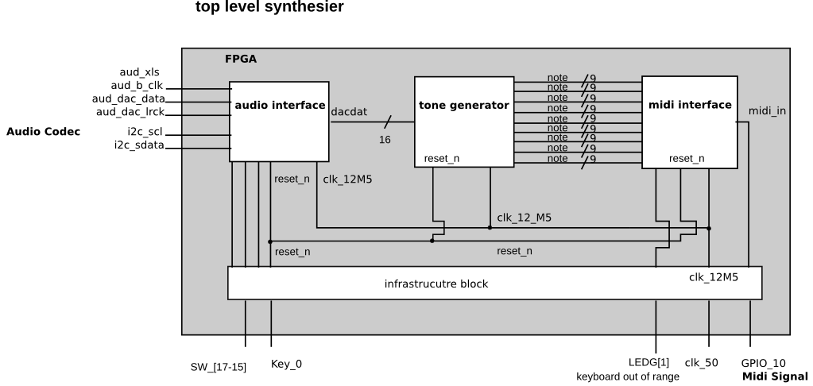
\includegraphics[width=0.9\textwidth]{images/midi_interface/top_synthesizer_block_saled.png}
	\caption{Top Synthesizer mit MIDI Interface: Blockschaltbild}
	\label{fig.top_synthesizer_block}
\end{figure}

Hier ist das Konzept der Umsetzung des MIDI Interface detaillierter beschrieben:

\begin{figure}[H]
	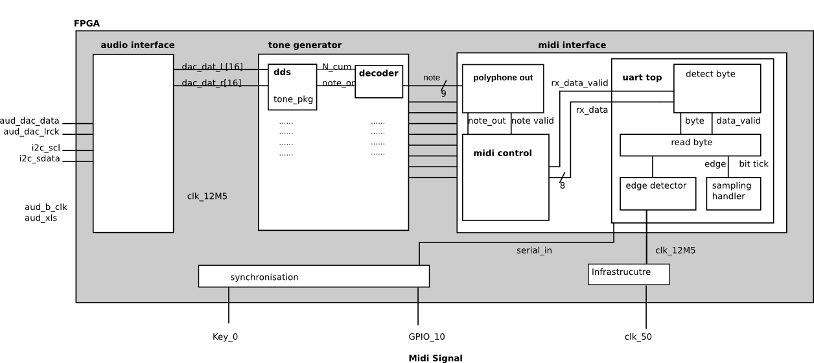
\includegraphics[width=0.9\textwidth]{images/midi_interface/top_synthesizer_detail_scaled.png}
	\caption{Top Synthesizer mit MIDI Interface: Detailansicht}
	\label{fig.top_synthesizer_detail}
\end{figure}

\chapter{RTL Top-Synthesizer}\label{chap.anhang_rtl_top_synthesizer}

\begin{figure}[H]
	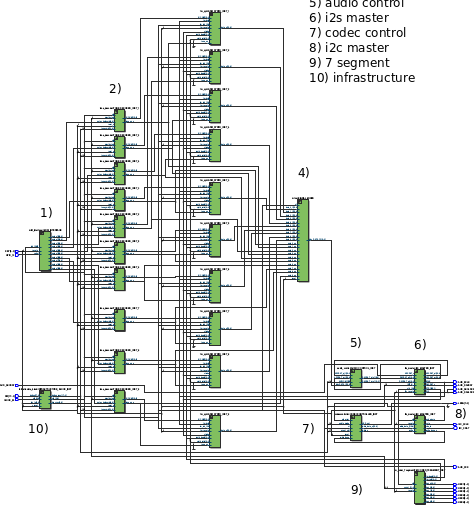
\includegraphics[width=0.9\textwidth]{images/midi_interface/RTL_10_Decoder_Mixwer.png}
	\caption{RTL Synthesizer-Projekt}
	\label{fig.rtl_top_synthesizer}
\end{figure}
	
	
	% add Bibliography to TOC
	%\addcontentsline{toc}{chapter}{\bibname}              
	%\bibliographystyle{plain}
	%\bibliography{BibTex/references}
	

\end{document}
%---------------------------------------------------------------------